\documentclass{article}
%\documentclass[a4paper,12pt,twoside]{book}
\usepackage{amsmath}
\usepackage{cite}
%\usepackage{tikz}
\usepackage{bm}
\usepackage{tikz,tkz-tab}
\usepackage{amsfonts}%
\usepackage{amssymb}%
\usepackage{hyperref}
\usepackage{mathtools}
%\usepackage{subcaption}
\usepackage{color}
\usepackage{multicol}
\usepackage{setspace}
\usepackage{empheq}
\usepackage{bbm, dsfont}
\usepackage{dsfont}
\usepackage{mathtools}
\usepackage{geometry}
\usepackage{enumitem} 
\usepackage[bottom]{footmisc}
\usetikzlibrary{arrows}
\usepackage{lscape}
\usepackage{tcolorbox}
\usepackage{caption}
%\usepackage{graphicx}
\usepackage{subfig}
\usepackage{multirow}
\usepackage{cite}
\usepackage{lscape}
\usetikzlibrary{shapes,snakes}
\renewcommand{\labelitemi}{$\bullet$}
\renewcommand{\labelitemii}{$\diamond$}

\usepackage{titlesec}
\usepackage[font=footnotesize,labelfont=bf]{caption}

\setcounter{secnumdepth}{4}

\titleformat{\paragraph}
{\normalfont\normalsize\bfseries}{\theparagraph}{1em}{}
\titlespacing*{\paragraph}
{0pt}{3.25ex plus 1ex minus .2ex}{1.5ex plus .2ex}


\newtheorem{definition}{Definition}

\usetikzlibrary{positioning}
\tikzset{main node/.style={circle,draw,minimum size=0.5cm,inner sep=0pt},
            }

%-------------------------------------------
\newtheorem{example}{Example}
\newtheorem{theorem}{Theorem}
\newtheorem{acknowledgement}[theorem]{Acknowledgement}
\newtheorem{algorithm}[theorem]{Algorithm}
\newtheorem{axiom}[theorem]{Axiom}
\newtheorem{case}[theorem]{Case}
\newtheorem{claim}{Claim}
\newtheorem{conclusion}[theorem]{Conclusion}
\newtheorem{condition}[theorem]{Condition}
\newtheorem{conjecture}[theorem]{Conjecture}
\newtheorem{corollary}{Corollary}
\newtheorem{criterion}[theorem]{Criterion}
\newtheorem{assumption}{Assumption}
\newtheorem{exercise}[theorem]{Exercise}
\newtheorem{lemma}{Lemma}
\newtheorem{observation}{Observation}
\newtheorem{notation}[theorem]{Notation}
\newtheorem{problem}[theorem]{Problem}
\newtheorem{proposition}{Proposition}
\newtheorem{remark}{Remark}
\newtheorem{solution}[theorem]{Solution}
\newtheorem{summary}[theorem]{Summary}
\newenvironment{proof}[1][Proof]{\textbf{#1.} }{\ \rule{0.5em}{0.5em}}




\begin{document}

\title{Preliminary Draft}

\maketitle

Title proposition 1: ``Big Tech is censoring me'': using social media data to verify the platforms' regulation policies regarding misinformation. 

Title proposition 2: Illustrating Facebook, Twitter and YouTube regulation policies against misinformation with a few chosen examples

Title proposition 3: Misinformation Policies of Mainstream Social Media Platforms: third-party verification methods and illustration

\tableofcontents

\section{Introduction}

Section $230$ in the United States Communications Decency Act provides immunity for website platforms against the content created by users. Similar regulations exist in the European Union via the E-commerce Directive (2000) in articles $12$ and $15$.\footnote{See section $4$ in Bayer (2019)~\cite{Bayer} for a comprehensive overview of the mentioned articles.} Nevertheless, there is growing pressure for Mainstream Social Media Platforms, such as Facebook, Twitter or Youtube, to moderate the available content. In particular, platforms take explicit actions when content is in violation of local laws in different jurisdictions, such as laws regarding defamation of a racial nature, dissemination of symbols from unconstitutional organizations, privacy protection, digital security, electoral laws. For example, Facebook reports having implemented a total of $64.7$ thousand content restrictions based on local law across all countries in 2020.\footnote{See Facebook Transparency Center, Content restrictions based on Local Law: \href{https://transparency.fb.com/data/content\-restrictions}{transparency.fb.com/data/content\-restrictions}. We summed the count of content restrictions over all countries reported in the table, for $H1$ and $H2$ of the year 2020.} %Google reports a total of $26$ thousand government requests to remove content from July 2020 to December 2020, among which $11.4$ thousand concerned Youtube.\footnote{See Google's Transparency report, government requests to remove content: \href{https://transparencyreport.google.com/government-removals/overview}{transparencyreport.google.com/government-removals/overview}.} Twitter reports having received $42.2$ thousand legal demands from third-parties from January to June 2020, and has responded by withholding $82$ thousand accounts and $3.1$ thousand tweets.\footnote{See Twitter Transparency website, Removal requests: \href{https://transparency.twitter.com/en/reports/removal-requests.html\#2020-jan-jun}{transparency.twitter.com/en/reports/removal-requests.html\#2020-jan-jun}.} 

\smallskip

Furthermore, mainstream platforms are increasingly engaging in editorial tasks by implementing targeted policies to insure that each platform's rules are not violated. Community guidelines of Facebook, Twitter and Youtube can be summarized in a handful of categories, regarding safety, privacy and authenticity; which include sub-categories such as violence, terrorism, child sexual exploitation, abuse, harassment, hateful conduct, suicide or self-harm, illegal or regulated goods and services, platform manipulation and spam (see table \ref{summary} in Appendix \ref{links}). While specific to each platform, the previously cited categories correspond in most cases to well defined concepts that fall into legal frameworks in many countries, unlike misinformation. The intricacies of constructing a legal framework for misinformation arises from the difficulty of identifying and qualifying a piece of online content as false or misleading, among an overwhelming quantity of daily produced content, without infringing existing laws.\footnote{See \href{https://www.poynter.org/ifcn/anti-misinformation-actions/}{A guide to anti-misinformation actions around the world} on the website of Poynter Institute.} In particular, a number of recent studies  point towards the idea that ``Fake News'' or disinformation is a small subset of the total supply of information on online social networking platforms (e.g. Grinberg et al. (2019)~\cite{grinberg} and Broniatowski et al. (2020)~\cite{broniatowski}). Yet, this seemingly small subset is generating great concern in traditional media and in society in a broader sense. \footnote{For example see the February 2020 \href{https://www.who.int/director-general/speeches/detail/munich-security-conference}{speech} of the Director General of the WHO at the Munich Security Conference, where he says ``But we’re not just fighting an epidemic; we’re fighting an infodemic.'' Furthermore, the European commission recognizes the spread of online disinformation as a problem and has put together in 2018 a \href{https://digital-strategy.ec.europa.eu/en/policies/code-practice-disinformation}{Code of practice on Disinformation}, which is a set of self-regulatory standards to fight disinformation. {\color{pink} Add more examples to show that this problem is highlighted by different institutions with different/neutral political color.. }}

\smallskip

In this article, we focus on mainstream platforms' policies and actions regarding content with low credibility or false information, commonly referred to as {\it Fake News} (for an overview of the concept see Lazer et al. (2018)~\cite{lazer}). The {\it Fake News} phenomenon is still ill-defined by the academic community, as it encompasses several combined features such as spreading inaccurate, false or misleading information, with or without the intention of influencing or manipulating a target pool of audience.  The growth of social networking platforms over the last decade in terms of number of users worldwide and volume of content, has modified the information ecosystem in terms of production of information and its mediation. Many users can now produce and share content which includes news related information, without having to abide by strict editorial processes that ensure accuracy of information and reliability of sources. In particular, false or inaccurate content produced and shared on social networking platforms concerning the political life or public health may have a potentially harmful impact on the society, in the rare event that it goes viral. This gave rise to a set of heterogenous fact-checking policies across mainstream platforms. For example, Facebook has a substantial partnership program with Fact-checking partners certified by the non-partisan International Fact-Checking Network. Facebook use a number of signals and machine learning models to predict misinformation and surface it to fact-checkers.\footnote{See the \href{https://www.facebook.com/journalismproject/programs/third-party-fact-checking/how-it-works}{section} Frequently asked questions: `How does Facebook use technology to detect potential misinformation?''} Twitter seems to have a different approach where they focus on providing context rather than fact-checking\footnote{To the best of our knowledge, Twitter does not have a page which summarizes its fact-checking strategy. The Twitter Safety Team tweeted on June 3, 2020 the following:  ``We heard: 1. Twitter shouldn’t determine the truthfulness of Tweets 2. Twitter should provide context to help people make up their own minds in cases where the substance of a Tweet is disputed. Hence, our focus is on providing context, not fact-checking.'' Tweet ID \href{https://twitter.com/TwitterSafety/status/1267986503721988096}{1267986503721988096}.} and the platform is testing a new system based on the wisdom of the crowds to tackle misinformation (see \href{https://blog.twitter.com/en\_us/topics/product/2021/introducing-birdwatch-a-community-based-approach-to-misinformation}{Twitter Birdwatch}). As for Youtube, this platform utilizes the \href{https://schema.org/ClaimReview}{schema.org ClaimReview} markup, where fact-checking articles created by eligible publishers can appear on information panels (see table \ref{summary} in Appendix \ref{links}).

\smallskip

During the COVID19 global health pandemic platforms have upgraded their guidelines to include a set of rules to tackle the propagation of potentially harmful content (see table \ref{summary} in Appendix \ref{links}). Those policies are enforced via existing actions used by the platforms to tackle other rules' violations, such as: labelling content to provide more context or indicate falsehood, publishing a list of terms or topics that will be flagged\footnote{{\color{pink} put here the list of Facebook and Twitter terms about covid.}}, suspending accounts, implementing strike systems, reducing the visibility of content, etc. As each platform is a private company, those {\it new} policies are not coordinated and are implemented in different ways across platforms. Such targeted policies show the willingness of mainstream platforms to enhance the quality of the online conversation, but also sheds light on the lack of specific policies to tackle misinformation in general. In particular, policies regarding misinformation are not part of the set of platform rules or community guidelines\footnote{As of July 2021.}. The 2019 report of the Facebook Data Transparency Advisory Group\footnote{To read the full report, see: \href{https://law.yale.edu/yls-today/news/facebook-data-transparency-advisory-group-releases-final-report?fbclid=IwAR2xMZr5GdD1GaNpjsXR3\_yeeIR4H9iFASfrni5HKcJVAO5oWA52bvwcZxU}{https://law.yale.edu/yls-today/news/facebook-data-transparency-advisory-group-releases-final-report?fbclid=IwAR2xMZr5GdD1GaNpjsXR3\_yeeIR4H9iFASfrni5HKcJVAO5oWA52bvwcZxU}.} (DTAG) states that ``{\it DTAG was not tasked with evaluating any of the following: (...) Facebook’s policies with respect to “fake news” or misinformation, as neither of these categories were counted as violations within the first two versions of the Community Standards Enforcement Report.}''. Facebook's strategy to tackle ``False News'' is three fold : Remove, Reduce, Inform. It is explained via a blog post on the facebook Newsroom.\footnote{See: \href{https://about.fb.com/news/2018/05/hard-questions-false-news/}{https://about.fb.com/news/2018/05/hard-questions-false-news/}.}. Similarly, Twitter communicates about actions related to misinformation via their Twitter Safety Blog/account\footnote{See \href{https://blog.twitter.com/en\_us/authors.TwitterSafety}{https://blog.twitter.com/en\_us/authors.TwitterSafety}.}. In a post on Youtube Official Blog\footnote{See \href{https://blog.youtube/inside-youtube/the-four-rs-of-responsibility-raise-and-reduce/}{https://blog.youtube/inside-youtube/the-four-rs-of-responsibility-raise-and-reduce/}.}, the platform explained its ``Four Rs of Responsibility" and how it raises authoritative content, reduces borderline content and harmful misinformation.  

\smallskip
 
%{\color{pink} Note, put here something along the following lines: cite misinformation review article about support for fact-checking + hard to correct beliefs once it goes viral. cite Pennycook / Rand? }
%In particular, determining the truthfulness of content over controversial topics or ongoing political events proves to be a tricky task and correcting beliefs about viral content, fact-checked as false ... 
%For an overview of Youtube's policy on fact-checking see: \href{https://support.google.com/youtube/answer/9229632}{support.google.com/youtube/answer/9229632}. To the best of our knowledge, Twitter does not have a page which summarizes its fact-checking strategy. The Twitter Safety Team tweeted on June 3, 2020 the following:  ``We heard: 1. Twitter shouldn’t determine the truthfulness of Tweets 2. Twitter should provide context to help people make up their own minds in cases where the substance of a Tweet is disputed. Hence, our focus is on providing context, not fact-checking.'' Tweet ID \href{https://twitter.com/TwitterSafety/status/1267986503721988096}{1267986503721988096}.} 
%In particular, the peculiar task of determining the truthfulness of content over controversial topics or ongoing political events 
%\smallskip

%{\color{pink} Note, put here something along the following line: make point here about the fact that in the transparency centers we find things for the violations in the platforms rules but not misinformation.... needed so that the academic community can study the reach and impact of this phenomena and provide guidelines for adequate actions... + where to put this \href{https://airtable.com/shrO0ooI9WSEfIUhb/tblAWQwFOiihKdQjm/viwZLAOzLK1NQ0c2n?blocks=hide}{airtable} ? }
%{\color{pink}  idea about academic community needs to be able to study this phenomenon and assess the impact of the policies, what effects they have etc. Violations fall into other categories: deceptive practices, impersonation, hate speech.  }

\begin{table}[]
\centering
\begin{tabular}{|l|c|l|l|l}

\hline
&  \begin{tabular}[c]{@{}l@{}} Application Programming Interface (API)  \end{tabular}                                                                                                                                                                                                                                                                                                                                                                                                                                            &    \multicolumn{1}{l|}{\begin{tabular}[c]{@{}l@{}} Web Scraping \end{tabular}}                                                                                                                                                                 \\ \hline
 
\includegraphics[scale=0.05]{./img/fb_logo.png} & \begin{tabular}[c]{@{}l@{}}\href{https://www.crowdtangle.com}{CrowdTangle API} and  \href{https://buzzsumo.com}{Buzzsumo API}   \end{tabular}                                                                                                                                                                                                               &      \multicolumn{1}{l|}{}    
\\ \hline
 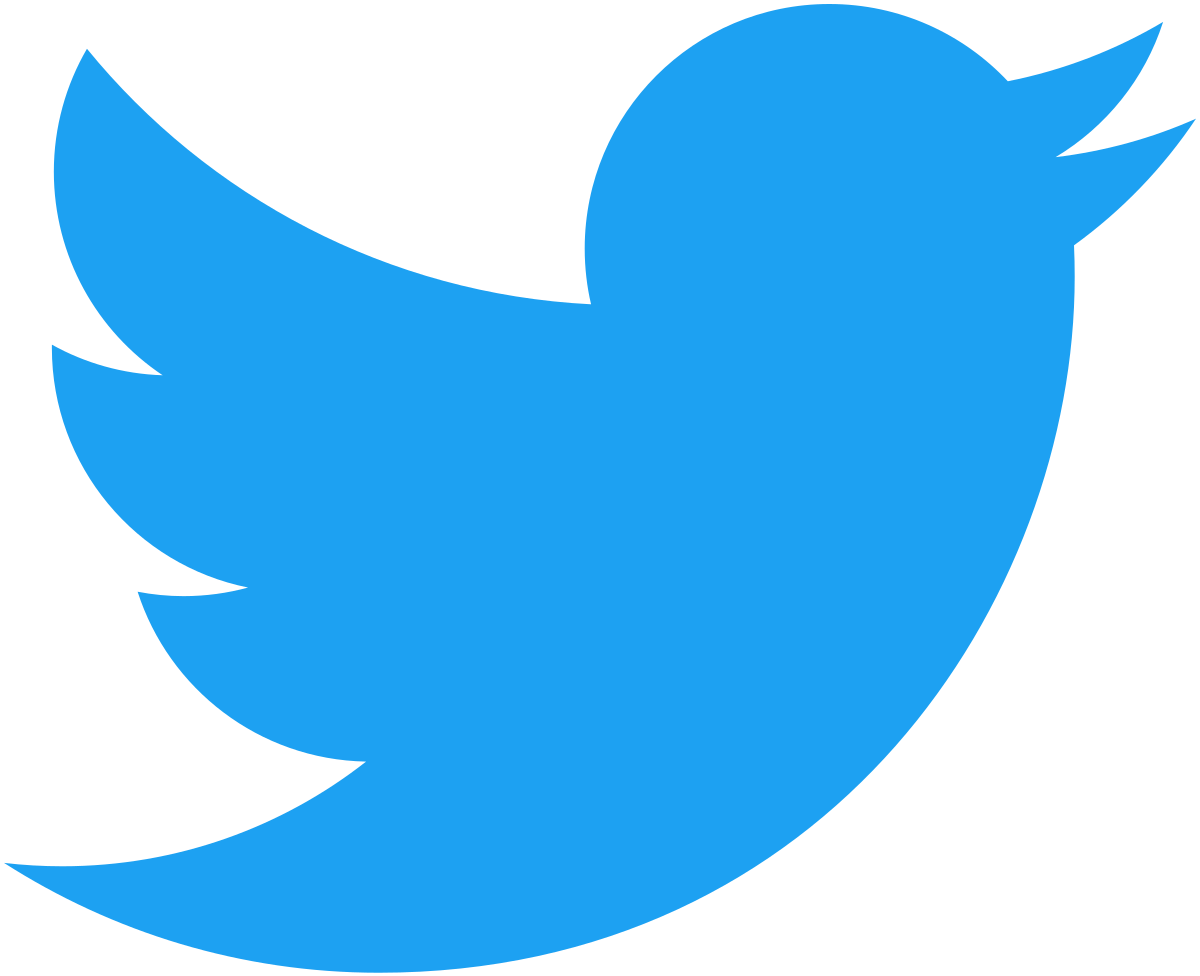
\includegraphics[scale=0.007]{./img/tw_logo.png}  &  \href{https://developer.twitter.com/en/docs/twitter-api/early-access}{Twitter API V2} & \multicolumn{1}{l|}{\href{https://github.com/medialab/minet/blob/master/docs/cli.md\#twitter-scrape}{Minet tw scrape}}                                                                                                                                                                           \\ \hline
 
\includegraphics[scale=0.03]{./img/yt_logo.png}  &  \href{https://developers.google.com/youtube/v3}{Youtube API V3}      &                                                                                                                            \multicolumn{1}{l|}{}                                                                                                                                                                           \\ \hline
\end{tabular}
\caption{Data collection}
\label{tab1}
\end{table}

Nevertheless, misinformation specific interventions by mainstream platforms are hard to monitor, study or verify by third parties (e.g. academic community, data journalists, NGOs), as in many cases misleading or false content does not qualify as a violation of a given platform's rules and it does not explicitly appear as a separate category in available transparency reports. This makes the study of online misinformation, the assessment of the impact of platforms' actions to tackle misinformation and their relevancy a burdensome task for the academic community. Hence, in the present article we explain how to verify with data mining mainstream platforms' current actions regarding content with low credibility or false information. We do so by providing a series of examples for different interventions and platforms. We only focus on three platforms: Facebook, Twitter and Youtube. Both Facebook and Youtube are in the top three most popular social media platforms in terms of number of users.\footnote{See for example the ranking of the most popular social networks as of April 2021 on Statista: \href{https://www.statista.com/statistics/272014/global-social-networks-ranked-by-number-of-users/}{https://www.statista.com/statistics/272014/global-social-networks-ranked-by-number-of-users/}.} We further choose Twitter because it is a social networking platform with the most news-focused users, according to the Pew Research center (2019)~\cite{pew1}. More specifically, we survey a number of common policies used in order to tackle misinformation, across the three above cited mainstream platforms, Facebook, Twitter and Youtube: temporary or permanent suspension of users, reducing the visibility of some content, introducing flags and notices. We do not provide  an exhaustive list of methods on how to investigate the platforms’ policies.\footnote{For a detailed list of interventions check the following \href{https://airtable.com/shrO0ooI9WSEfIUhb/tblAWQwFOiihKdQjm/viwZLAOzLK1NQ0c2n?blocks=hide}{airtable} compiled by Slatz and Leibowicz (2021)~\cite{niemanlab}. } We rather provide a methodology to investigate key policies, that can be useful to researchers or journalists interested in implementing external monitoring. We summarize in table \ref{tab1} the tools used to collect the data from Facebook, Twitter and Youtube, that we use in multiple examples throughout the present article. We compile in Appendix \ref{links} in table \ref{summary}, URL links that redirect to the policies, regulations and transparency centers of Facebook, Twitter and Youtube. Finally, we discuss how an increased effort of transparency regarding specific content can help the community of researchers study and assess the impact of platforms' policies regarding misinformation.  %the announced policy for a specific user was implemented or not.  

%Second, we provide simple means to check how those policies are implemented in practice and discuss how to assess their impact, when possible. 

%We do not aim for an exhaustive list of methods on how to investigate the platforms’ policies against misinformation, but rather to share the methods we currently know, and that we think can be useful to researchers or journalists interested in that question. We are aware that other APIs or databases can be useful on that matter, but we will only mention here the ones about which we have some experience.

%\bigskip

%{\color{red} Policies not specific to misinformation, but to enforce laws + things already used for terrorism and hate speech. Intro or/and Discussion. accounts: hard to say suspension for which.} 
% Misinformation : which law ? not defined ! 
%: Public content insights tool owned and operated by Facebook.
%\footnote{Public content insights tool owned and operated by Facebook.}
%: commercial content \\ database




 %We We are aware that other APIs or databases can be useful on that matter, but we will only mention here the ones about which we have some experience.
%CrowdTangle is a public insights tool owned and operated by Facebook, that exclusively tracks public content from Facebook public groups and pages. BuzzSumo is a commercial content database that tracks the volume of user interactions with internet content on Facebook, Twitter, and other social media platforms. 
%Section 230 in the US + EU 
%Pressure to moderate and mix-up of platforms with public square… 
%Rôle dans la production/médiation : P-M-R 
%Pourquoi faut-il vérifier leurs politiques ? D’une part parce que ce sont les plateformes elles-mêmes qui annoncent leurs effets. D’autre part beaucoup de choses indirectes. 
%Add disclaimer in a footnote early on in the document : document not meant to be an exhaustive overview of all the existing regulations and point to three or four main legal sources for exhaustive references. 
%Such policies include the introduction of notices (Twitter, see link) or flags (Facebook, see…) to signal to users inaccurate or false content, the temporary or permanent suspension of accounts (Twitter) or pages (Facebook), reducing the visibility of posts or pages (Facebook), or blocking users from sharing specific URL links (see link). The objective of this article is twofold. First, we study the impact of a number of  implemented measures by mainstream platforms to tackle (mis)disinformation. 


\section{Temporary \& permanent suspension}

Mainstream social media platforms may suspend the account of a specific user when they deem that the platforms' rules have been violated. Account suspension can be temporary or permanent.\footnote{A list of notable Twitter temporary and permanent suspensions can be found on wikipedia: \href{https://en.wikipedia.org/wiki/Twitter_suspensions}{https://en.wikipedia.org/wiki/Twitter\_suspensions}.}  When the suspension is temporary the user is prohibited for a limited period of time from posting content on their account, but created content prior to suspension remains available to the user and their followers. However, when the suspension is permanent, in most cases, followers or subscribers have no longer access to the content prior to the suspension and the user can no longer use the account to create new content.  In what follows, we focus on the implementation of this policy by several platforms and provide simple examples to illustrate. 

\subsection{Facebook}

When an account is permanently suspended by Facebook, it disappears from the platform. That is,  the data can no longer be scrapped and it also disappears from the CrowdTangle API.\footnote{CrowdTangle is a public insights tool owned and operated by Facebook, that exclusively tracks public content from Facebook public groups and pages.} Facebook publishes on monthly basis a {\it coordinated inauthentic behavior} report, where it informs how many personal accounts, pages or groups were deleted and to which {\it deceptive network} they may have belonged to.\footnote{See the \href{https://about.fb.com/news/2021/05/april-2021-coordinated-inauthentic-behavior-report/}{April 2021 report} as an example.} But as long as external persons do not have access to deleted accounts data, these reports cannot be verified by independent researchers or journalists.

\begin{figure}[h]
	\centering
		%\begin{multicols}{1}
			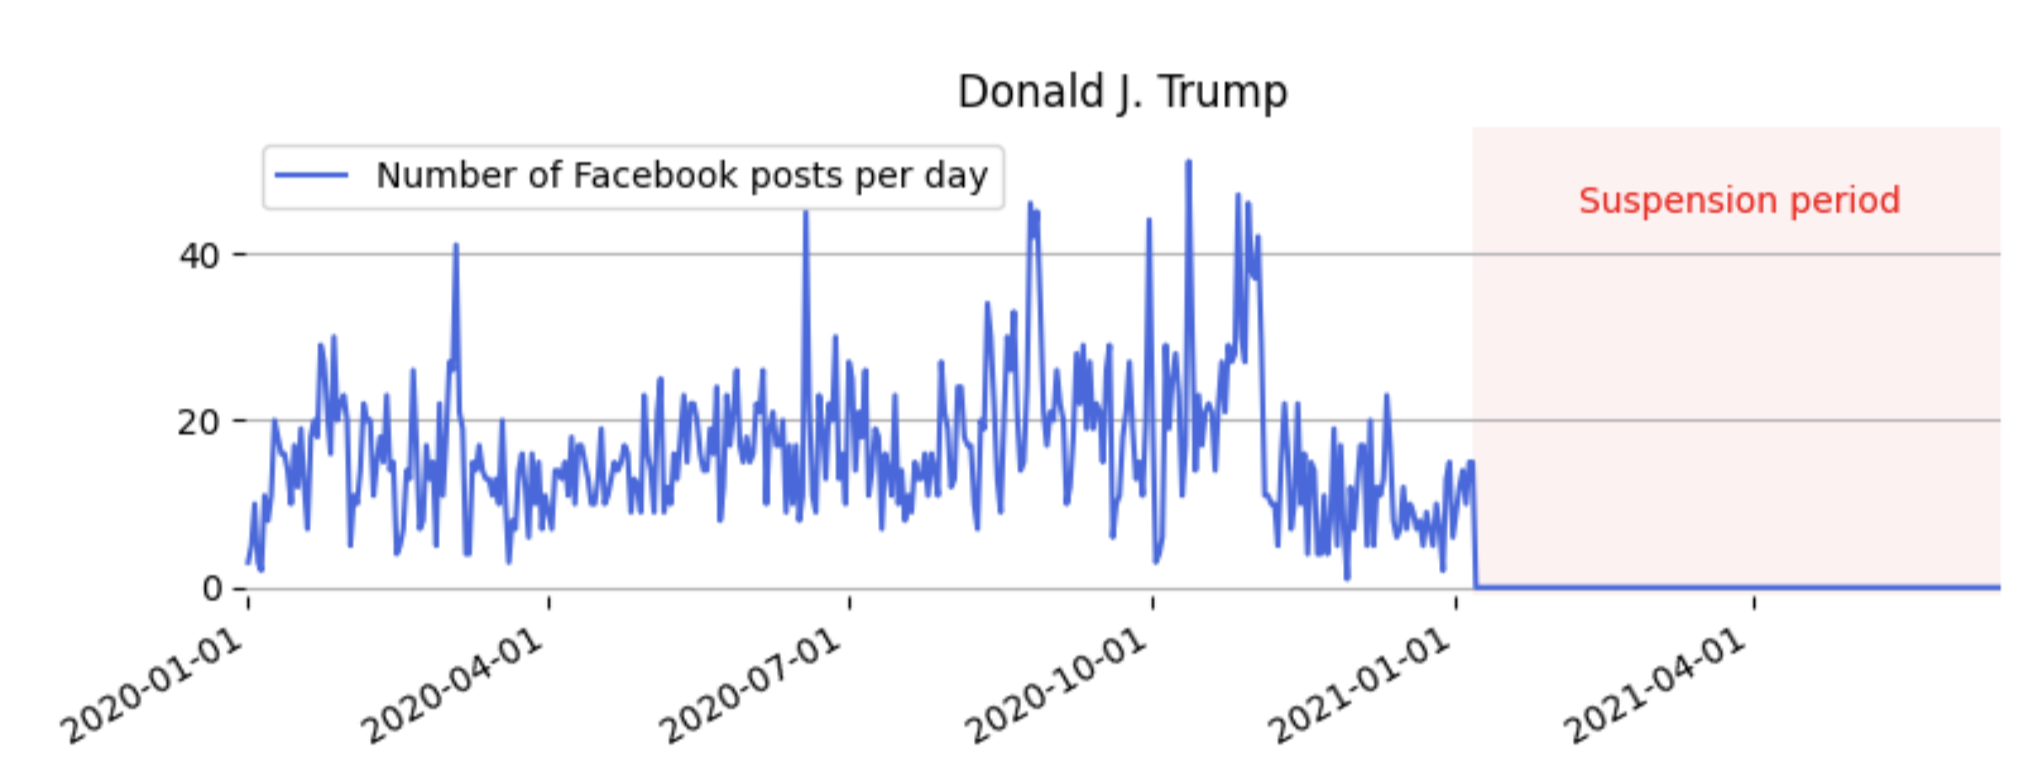
\includegraphics[scale=0.3]{./img/fb/fig1_fb.png}
		%\end{multicols}
	\caption{Number of Facebook posts published each day by the Facebook page {\it Donald J. Trump} between January $1$, $2020$ and June $15$, $2021$. The data corresponds to $6$ $083$ posts retrieved from the CrowdTangle API using the {\it posts} endpoint.}
	\label{fig1_fb}
\end{figure}

Facebook can also apply a temporary suspension, and in this case the data can often be collected and analyzed. For example, \href{https://www.facebook.com/DonaldTrump/}{Donald Trump’s official Facebook page}  has been suspended following the Capitol attack on January 6, 2021.\footnote{See \href{https://www.facebook.com/zuck/posts/10112681480907401}{https://www.facebook.com/zuck/posts/10112681480907401}} Nevertheless the page’s data is still present in the CrowdTangle API. Thus, after manually adding this page to the CrowdTangle dashboard, we collected the $6$ $083$ posts it had published between January $1$, $2020$ and June $15$, $2021$ using the {\it posts} endpoint.\footnote{See the endpoint documentation for more details: \href{https://github.com/CrowdTangle/API/wiki/Posts}{https://github.com/CrowdTangle/API/wiki/Posts}.} We used Minet command line tool \cite{minet} to collect the data.\footnote{The exact command can be found \href{https://github.com/medialab/truth-and-trust-online-2021/blob/master/code/collect_facebook_crowdtangle_trump_data.sh}{here}.} We can verify on figure \ref{fig1_fb} that the {\it Donald J. Trump} page has not published any content since January $6$, 2021, and that this behavior is not consistent with the page’s previous activity: an average of $16$ posts were published each day on Facebook before the suspension. 

\subsection{Twitter}

%paragraph strike system + say following example is a manual decision. 
Twitter has implemented a strike system as part of their Civi Integrity Policy\footnote{See \href{https://help.twitter.com/en/rules-and-policies/election-integrity-policy}{help.twitter.com/en/rules-and-policies/election-integrity-policy}} and their COVID19 misleading information policy.\footnote{See \href{https://help.twitter.com/en/rules-and-policies/medical-misinformation-policy}{help.twitter.com/en/rules-and-policies/medical-misinformation-policy} and \href{https://blog.twitter.com/en\_us/topics/company/2021/updates-to-our-work-on-covid-19-vaccine-misinformation}{blog.twitter.com/en\_us/topics/company/2021/updates-to-our-work-on-covid-19-vaccine-misinformation}} Violations of both policies can entail strikes, where two strikes lead to a 12-hour account lock and five or more strikes lead to permanent suspension from the platform. The 12-hour account lock is hard to observe in the data, especially for users who do not have an over the clock tweeting activity. In this section, we provide one example of a temporary suspension\footnote{See the official documentation on the Twitter's Help Center regarding account suspension: \href{https://help.twitter.com/en/managing-your-account/suspended-twitter-accounts}{https://help.twitter.com/en/managing-your-account/suspended-twitter-accounts }.} of a Twitter account, that seems to be the result of a manual decision concerning a Tweet which violated the rules. 

The Twitter account $@LifeSite$ of the website lifesitenews.com has been suspended for at least two periods of time: from end of 2019 until fall 2020 for 308 days, then again since January 2021 for having violated Twitter Rules\footnote{See Lifesitenews's article discussing the reason for the suspension: \href{https://www.lifesitenews.com/news/lifesite-is-dumping-twitter-and-so-should-you}{https://www.lifesitenews.com/news/lifesite-is-dumping-twitter-and-so-should-you}. Twitter rules can be found at: \href{https://help.twitter.com/en/rules-and-policies/twitter-rules}{https://help.twitter.com/en/rules-and-policies/twitter-rules}. }. In particular, this website has several failed fact-checks concerning the published articles, according to Iffy.news.\footnote{See \href{https://mediabiasfactcheck.com/life-site-news/}{https://mediabiasfactcheck.com/life-site-news/}}. We collected the activity (tweets, replies, quotes, retweets) on their Twitter account via the Twitter API, using the historical search endpoint.\footnote{See the documentation: \href{https://developer.twitter.com/en/docs/twitter-api/tweets/search/api-reference/get-tweets-search-all}{https://developer.twitter.com/en/docs/twitter-api/tweets/search/api-reference/get-tweets-search-all}.} We then plotted the number of Tweets, Retweets, Quotes and Replies per day, as shown in panel $a$ of figure \ref{fig2}). The two periods of temporary suspension are clearly observed in the data as the user(s) of the account were not allowed to use the functionalities of the Twitter Platform. 

\begin{figure}[h]
\centering
	%\begin{multicols}{1}
		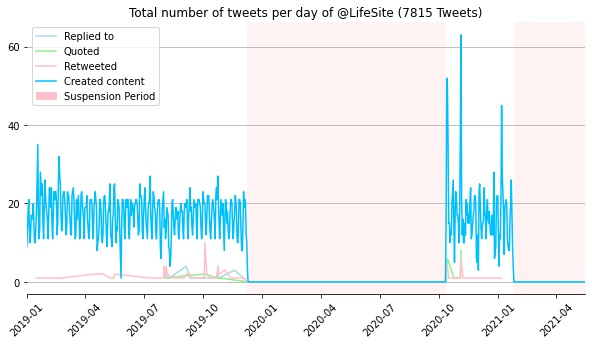
\includegraphics[scale=0.35]{./img/lifesite.jpg} 
	%\end{multicols}
	%\begin{multicols}{1}
		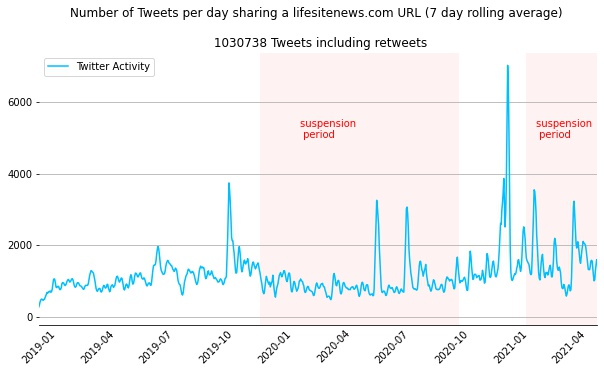
\includegraphics[scale=0.35]{./img/lifesite_rolling_7_lifesite.jpg}
	%\end{multicols}
\caption{Panel (a): number of Tweets per day of the Twitter account $@Lifesite$ linked to the website lifesitenews.com from January, 2019 until April 2021. Panel (b): number of Tweets per day that have shared a lifesitenews.com URL link from January, 2019 until April 2021. }
\label{fig2}
\end{figure}

To further assess the impact of this double temporary suspension, we collect via Minet Command Line Tool\cite{minet}, all the tweets that have shared during the same period a url link containing lifesitenews.com. Panel $(b)$ of figure \ref{fig2}, shows that during both periods of temporary suspension, other users still shared lifesitenews.com links and that the level was only slightly below the tweeting and retweeting levels prior to the first temporary suspension. More specifically, there was an average of 960 tweets (including retweets) per day over the first temporary suspension period of 308 days from December 9, 2019 until October 12, 2020, against an average of 977 tweets (including retweets) per day during the exact same period one year earlier. Finally, panel $(b)$ points towards the limitations of suspending an account to limit the spread of its content. 

\subsection{Youtube}

In this section, we turn to the channel's temporary or permanent suspension policy of Youtube. Whenever a channel publishes a video that violates the community guidelines for the first time they will  usually receive a warning and the content will be removed. For the second time the channel will start receiving strikes. A first strike results in limiting the access of the Youtube channel  for one week, like uploading videos, streaming and other activities. Then a second strike is similar but the suspension will be for two weeks. A third strike results in the termination of the channel. The strike count of a channel lasts 90 days.  In the special case, where a video is in extreme violation of the guidelines, the publishing channel may get terminated without a warning.\footnote{See the ``Community Guidelines strike basics''. Youtube help, Google Developers,  \href{https://support.google.com/youtube/answer/2802032?hl=en. Accessed 21 6 2021}{https://support.google.com/youtube/answer/2802032?hl=en. Accessed 21 6 2021}.} To illustrate the implementation of this policy we provide two examples for the temporary suspension of the following two Youtube channels: \href{https://www.youtube.com/channel/UCNbIDJNNgaRrXOD7VllIMRQ}{One America news Network} and \href{https://www.youtube.com/user/TonyHeller1}{Tony Heller}.

\begin{figure}[h]
	\centering
	%\begin{multicols}{1}
		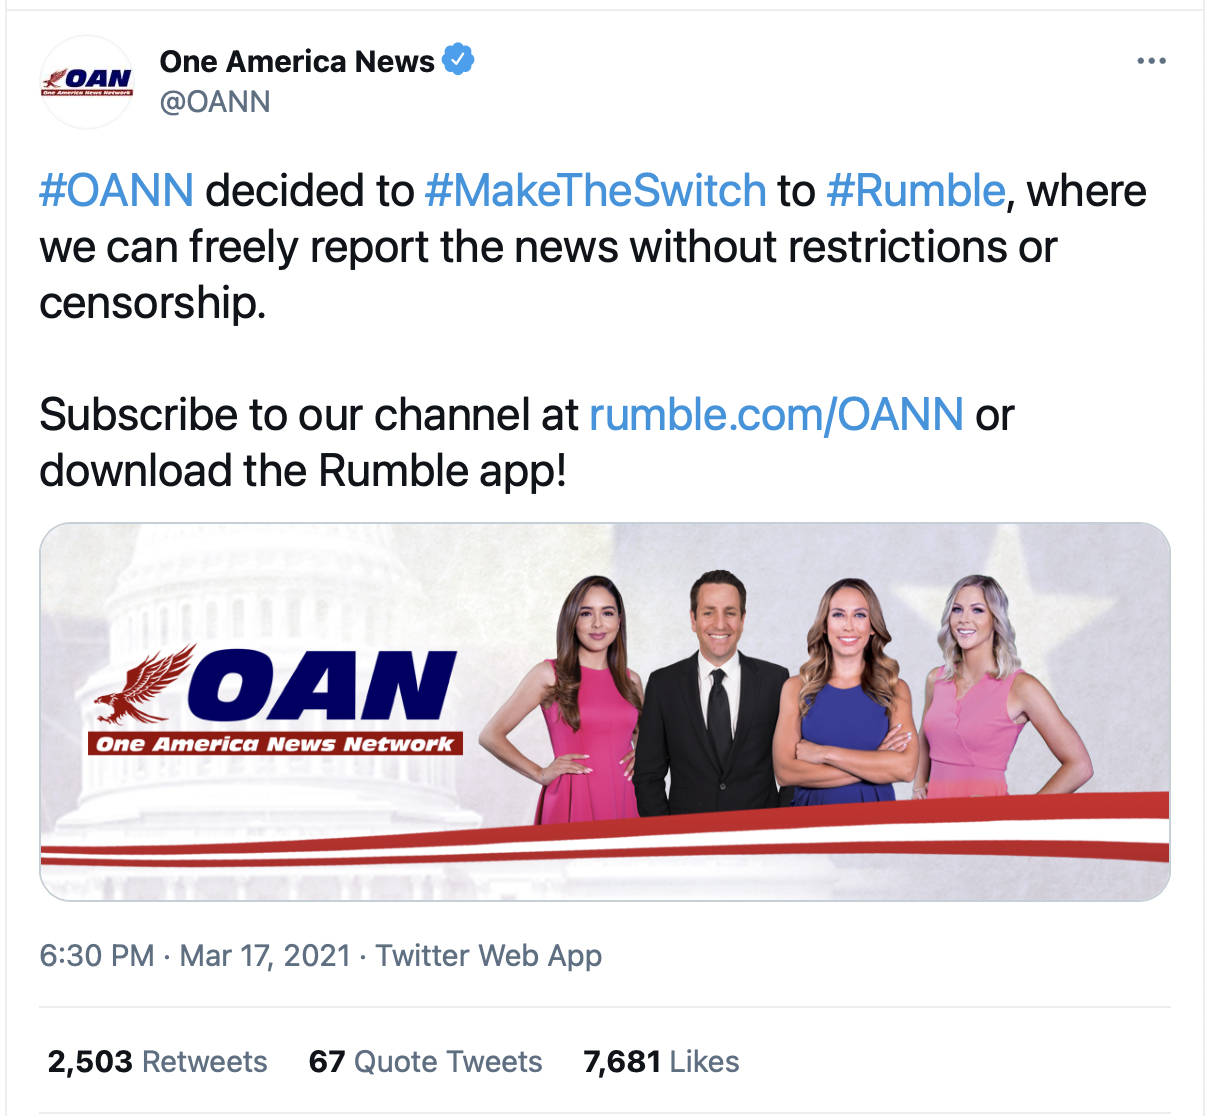
\includegraphics[scale=0.21]{./img/oann/fig3_oann.png}
	%\end{multicols}
	%\begin{multicols}{1}
		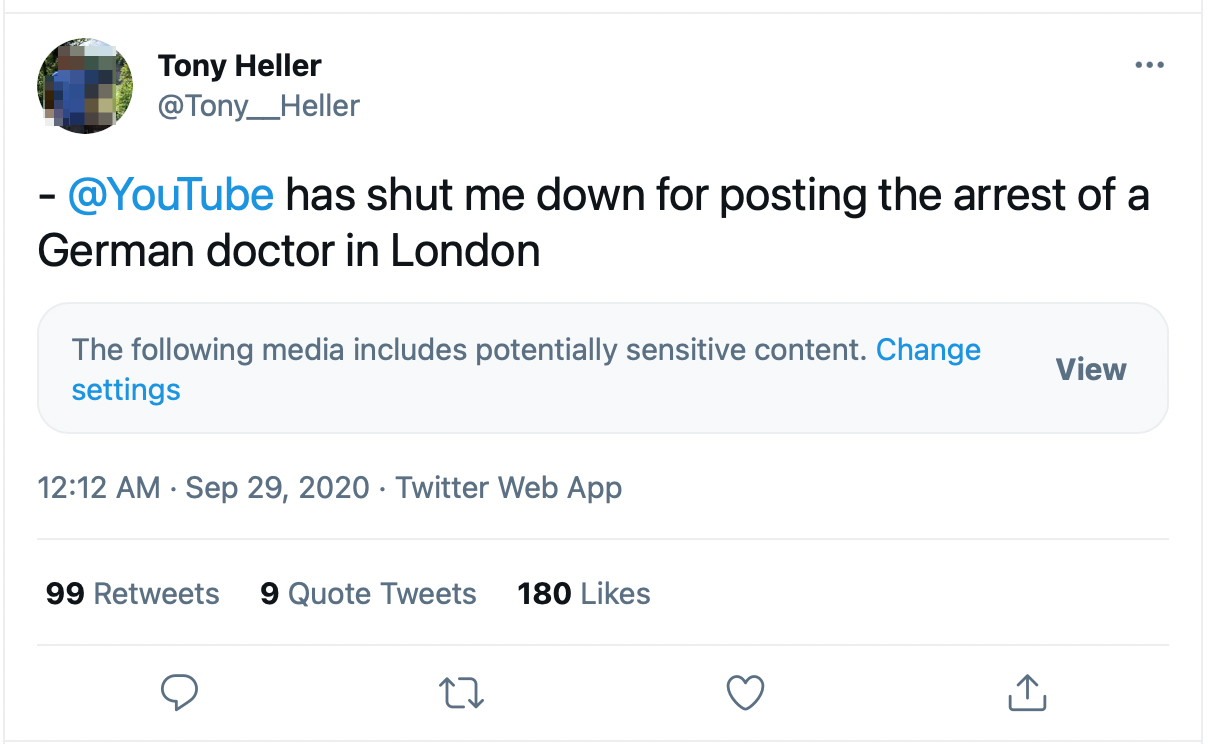
\includegraphics[scale=0.31]{./img/tony/fig3_tony.png}
	%\end{multicols}
	
	\caption{Panel (a): Tweet announcing moving to rumble by OANN (Twitter), Twitter ID \href{https://twitter.com/OANN/status/1372238828425998336}{1372238828425998336}. Panel (b): Tony Heller's tweet after getting suspended from Youtube, Twitter ID \href{https://twitter.com/Tony\_Heller/status/1310703852769796097}{1310703852769796097}.}
	\label{fig2_oann}
\end{figure}

%\smallskip

First, we investigate the temporary suspension case of the Youtube Channel of {\it One America News channel}. This channel received a first strike on November 24, 2020 for the promotion of  a false cure for COVID19.\footnote{See nbcnews,  \href{https://www.nbcnews.com/news/all/youtube-suspends-oann-violating-its-covid-19-policy-n1248845}{YouTube suspends OANN for violating its Covid-19 policy} nbcnews, Ahiza García-Hodges, 24 11 2020.} We collected the activity of the channel OANN (video counts, view counts) using  the Youtube API v3, between November 2020 and January 2021. For the video counts, we used the playlist endpoint to retrieve the videos uploaded with their publishing date and for the view count we used the IDs of the videos we had from the playlists and via the videos endpoint we retrieved the view counts on June 2021.\footnote{See the Google documentation  \href{https://developers.google.com/youtube/v3/docs/videos/list}{https://developers.google.com/youtube/v3/docs/videos/list} and \href{https://developers.google.com/youtube/v3/docs/playlists/list}{https://developers.google.com/youtube/v3/docs/playlists/list}} 

\begin{figure}[h]
	\centering
	%\begin{multicols}{1}
		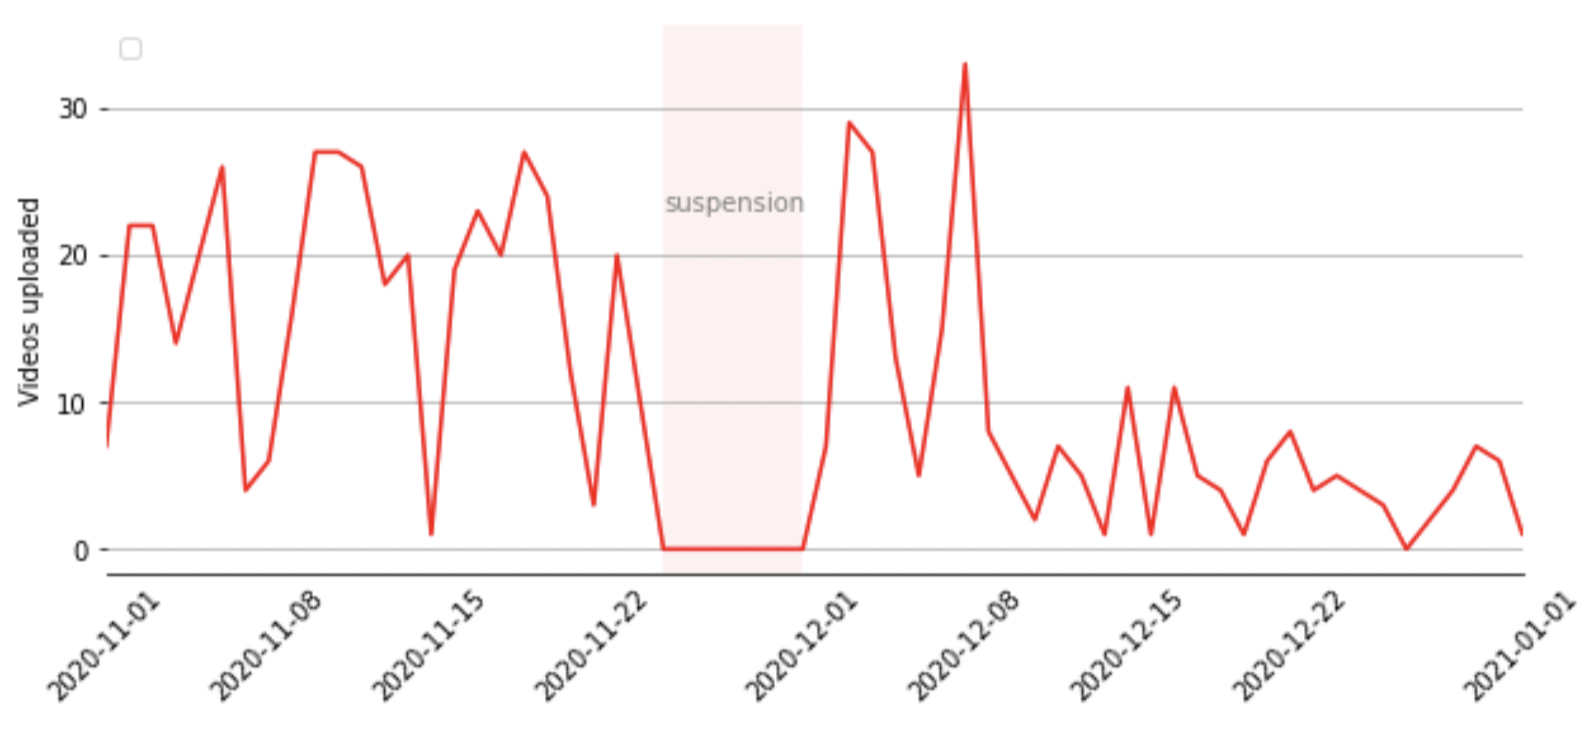
\includegraphics[scale=0.27]{./img/oann/fig1_oann.png}
	%\end{multicols}
	%\begin{multicols}{1}
		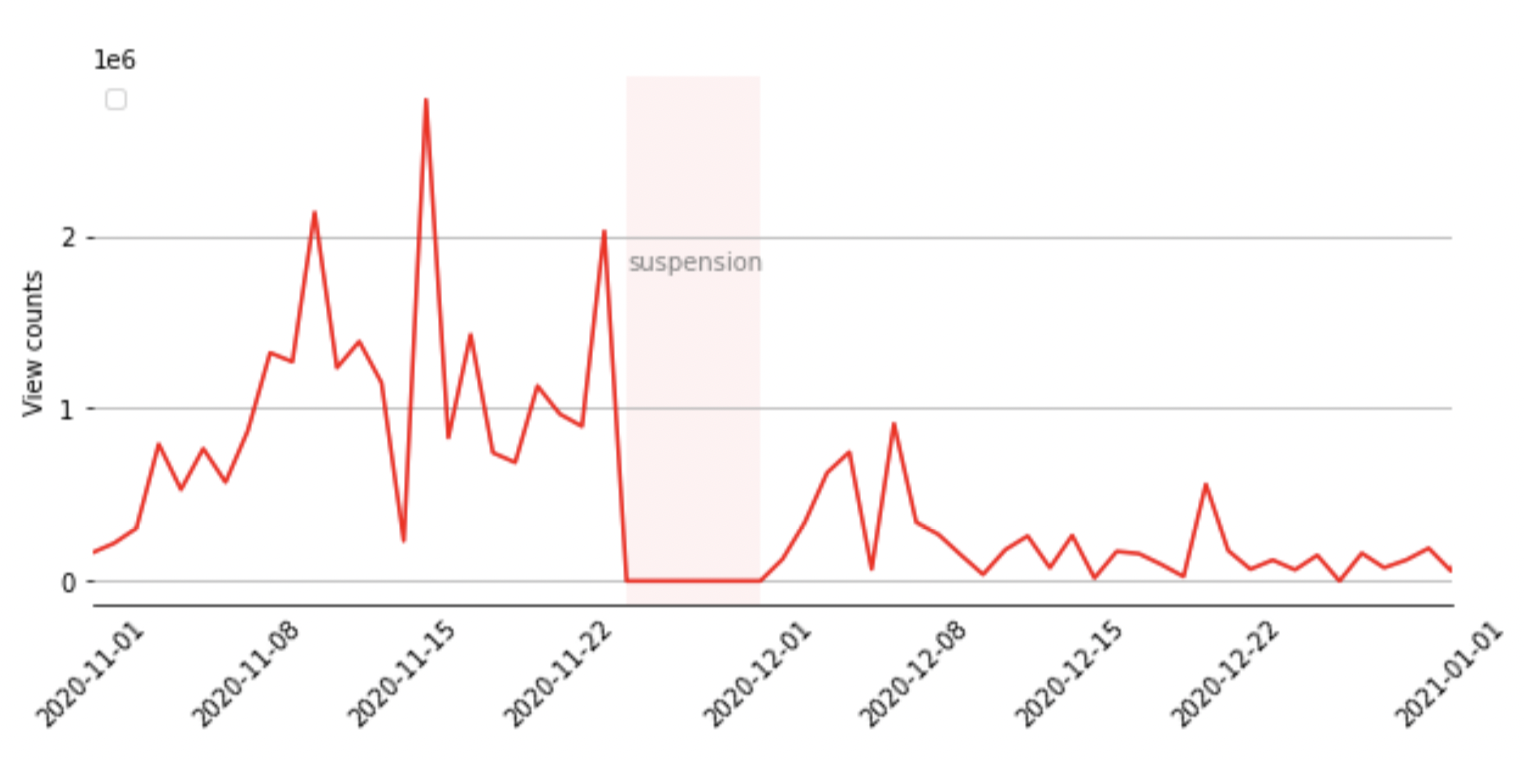
\includegraphics[scale=0.26]{./img/oann/fig2_oann.png} 
	%\end{multicols}
	\caption{panel (a): Number of Youtube videos uploaded each day by the youtube channel {\it One America news Network} November 1, 2020 and January 1, 2021. Panel (b): accumulated view counts for videos. The metrics correspond to the videos’  publishing date and the data is retrieved from the youtube API with the {\it playlists} and  {\it videos} endpoints. }
	\label{fig1_oann}
\end{figure}


In addition, as shown in figure \ref{fig1_oann} when comparing the month before the suspension from 2020/10/24 to 2020/11/24 and one month after from 2020/12/01 to 2021/01/01 it was found that the view count decreased by -73\% and the videos uploaded by -55\%. Besides that, OANN decided to move officially to Rumble on March 17, 2021 as announced on their Twitter account (see figure \ref{fig2_oann}) and their upload activity on their Youtube channel is close to zero since that announcement. 

%\smallskip
\begin{figure}[h]
	\centering
		%\begin{multicols}{1}
			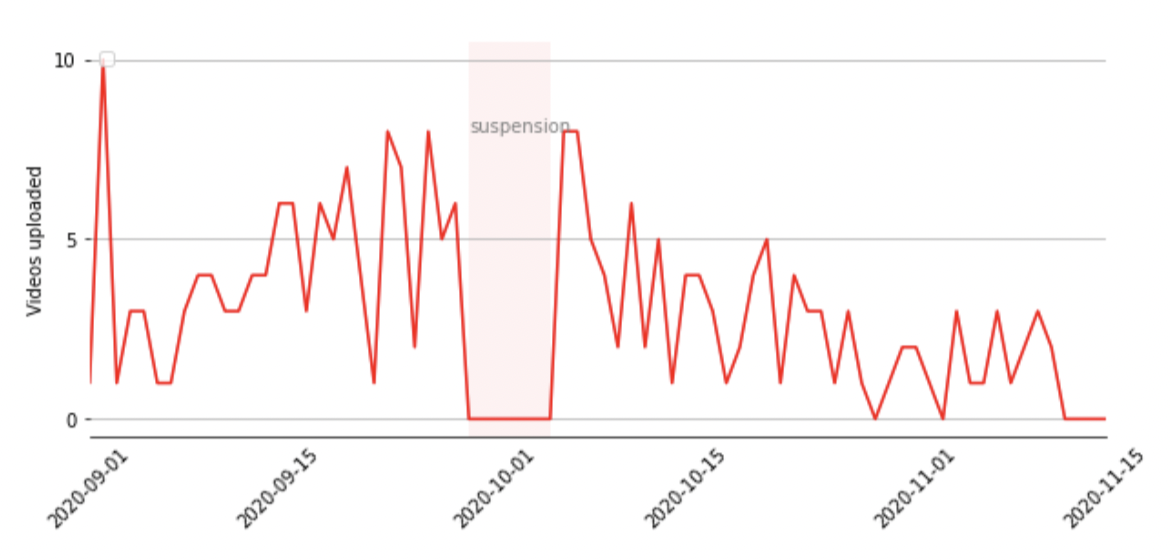
\includegraphics[scale=0.35]{./img/tony/fig1_tony.png}
		%\end{multicols}
		%\begin{multicols}{1}
			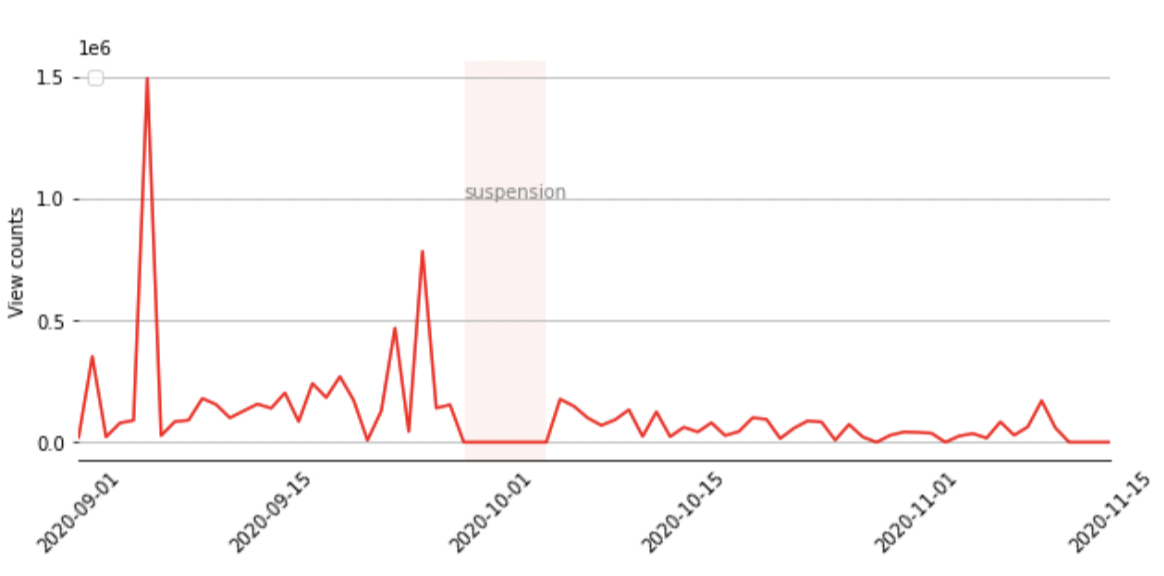
\includegraphics[scale=0.34]{./img/tony/fig2_tony.png}
		%\end{multicols}
	\caption{Panel (a): Number of Youtube videos uploaded each day by the Youtube channel {\it Tony Heller} between September 1, 2020 and November 15, 2020. Panel (b): accumulated view counts for videos uploaded by the same Youtube channel. The date corresponds to the videos’  publishing date. 
}
	\label{fig1_tony}
\end{figure}

We now turn to our second example, the temporary suspension of the Youtube channel Tony Heller. This channel got its first strike after posting a video about an anti-covid-lockdown doctor getting arrested (see screenshot in figure \ref{fig2_oann}). The suspension period was for one week from September 29 until October 5. We applied the same methods as in the previous example for the data collection. Figure \ref{fig2_oann} shows the daily number of videos uploaded by the channel. The suspension period can be observed clearly in the historical data of the channel.  observing the reach of the audience 
Figure 3: Tony heller tweet after getting suspended from youtube (Twitter)
using view counts one month before the suspension starting from 2020/08/28 to 2020/09/28 and one month after the suspension from 2020/10/05 to 2020/11/05 the channel witnessed a drop of view counts by $-69.5\%$ and the videos published in the channel were less by $-29\%$. This drop in views can show that the  suspension  period
may  have  a  good  impact  on  reducing  the  audience interest or reach to the channel.

%%%%%%%%%%%%%%%%%%%%%%%%%%%%%%%%%%%%%%%%%%%%%%%%%%%%%%%%%%%%%%%

\section{Flags, Notices and labels}

\subsection{Facebook}

To the best of our knowledge, two types of flags can currently be seen on Facebook posts, videos and pictures: $(i)$ information banners that do not refute the message in the post but that give a link to an authoritative source, such as ``Visit the COVID-19 Information Centre for vaccine resources'' and $(ii)$ fact-check flags that provide a ``judgement'' on the text of the post or the link, shared, such as ``False information Checked by independent fact-checkers'' (see Figure \ref{fb_flags}). The fact-check flags can be of varied nature : `False', `Partly false', `Missing context', `False headline', `Altered media', `Opinion', `Satire', `Not eligible' and even `True'.

\begin{figure}[h]
\centering
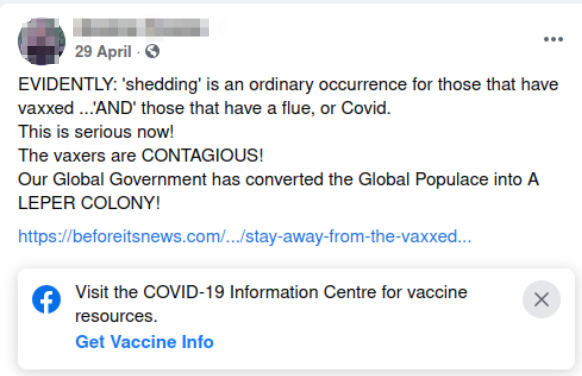
\includegraphics[scale=0.35]{./img/fb_flags/fb_flag_1.png}
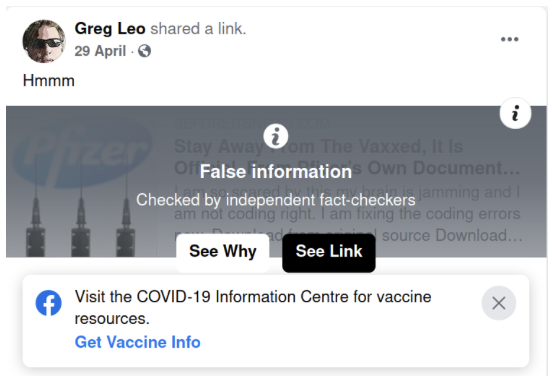
\includegraphics[scale=0.35]{./img/fb_flags/fb_flag_2.png}
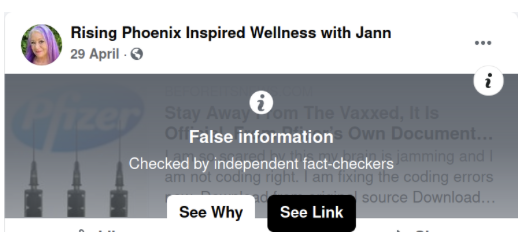
\includegraphics[scale=0.49]{./img/fb_flags/fb_flag_3.png}
\caption{Examples of Facebook posts having shared a link fact-checked as False by one of Facebook’s partners. Screenshots taken on July 8, 2021: \href{https://www.facebook.com/groups/1220117708132394/permalink/2386760061468147}{facebook.com/groups/1220117708132394/permalink/2386760061468147},  \href{https://www.facebook.com/groups/473809623000471/permalink/1333200093728082}{facebook.com/groups/473809623000471/permalink/1333200093728082}, \href{https://www.facebook.com/691911990845585/posts/3835629366473816}{facebook.com/691911990845585/posts/3835629366473816}).} 
\label{fb_flags}
\end{figure}

No information regarding the flags can be found on Buzzsumo or CrowdTangle, the two APIs we use to access Facebook data. The only way to verify Facebook’s flag policy is thus to scrap Facebook. For this paper, we added a new feature in minet to scrape Facebook posts and automatically verify for the presence of the flags.

We first searched for all the Facebook posts having shared a link rated as ‘False’ by Science Feedback with the {\it search} endpoint in minet\footnote{ link: \href{https://beforeitsnews.com/eu/2021/04/stay-away-from-the-vaxxed-it-is-official-from-pfizers-own-documents-2671454.html}{https://beforeitsnews.com/eu/2021/04/stay-away-from-the-vaxxed-it-is-official-from-pfizers-own-documents-2671454.html} and its fact-check: \href{https://healthfeedback.org/claimreview/insufficient-evidence-to-claim-covid-19-vaccines-cause-menstrual-irregularities-in-vaccinated-women-vaccinated-people-arent-making-unvaccinated-people-ill/}{https://healthfeedback.org/claimreview/insufficient-evidence-to-claim-covid-19-vaccines-cause-menstrual-irregularities-in-vaccinated-women-vaccinated-people-arent-making-unvaccinated-people-ill/}).}. Twenty Facebook posts were collected this way, and the newly developed scraper was used to verify whether they were flagged with an information banner, a fact-check flag, both or none. Three posts were unavailable, and thus could not be categorized by the scraper. As Science Feedback has sent a False fact-check for this link to Facebook, we would expect all these posts to contain a fact-check flag, but we had no expectations for the information banner. 

\smallskip

Surprisingly only $11$ posts out of the remaining $17$ had a ‘False information’ flag  (Table \ref{tab_flags_fb}, see left panel of Figure \ref{fb_flags} for an example). We observed that the flagged posts were also the ones in which the false link was expanded (i.e., a banner was visible with an image of the link and that can be clicked on, see the middle and right panels of Figure \ref{fb_flags} for examples). As the ‘False information’ flag is applied on the link banner, and not on the link itself, a user is thus able to share a False link on Facebook without the ‘False information’ banner if the link is not expanded.

\begin{table}[h]
\begin{tabular}{|c|c|c|c|}
\hline
\multicolumn{4}{|c|}{Number of posts}                                                                                                                    \\ \hline
with no flag & with an information flag & with a fact-check flag & \begin{tabular}[c]{@{}c@{}}with a fact-check and an \\  information flags\end{tabular} \\ \hline
0            & 7                        & 4                      & 7                                                                                     \\ \hline
\end{tabular}
\caption{Count for the Facebook posts with the different types of flags having shared a link fact-checked False by one of Facebook’s partners}
\label{tab_flags_fb}
\end{table}

We also observed that most of the posts sharing this False link (13 out of 17, Table \ref{tab_flags_fb}) had an information banner saying ‘Visit the COVID-19 Information Centre for vaccine resources’ (see the first two examples of Figure \ref{fb_flags}). We could not identify why the banner was applied on some posts and not on others (we saw no clear difference in the post messages for example). It should be noted that some posts displayed both the information and the fact-check banners, as in the middle panel of Figure \ref{fb_flags}.

\subsection{Twitter}

Alongside other social networking platforms, when the content of a tweet violates the Twitter rules, a notice can be added to provide more context according to Twitter's Help Center.\footnote{See Notices on Twitter and what they mean: \href{https://help.twitter.com/en/rules-and-policies/notices-on-twitter}{https://help.twitter.com/en/rules-and-policies/notices-on-twitter}.} At the tweet level, notices take the form of a label or an interstitial. Labels are context specific (e.g. COVID19 or presidential elections) and  redirect users to a URL to get more context, for example ``Get the facts about COVID-19'' (see right panel of figure \ref{fig8}). Interstitials are presented as a greyed box on top of a tweet, which indicate sensitive content, violations of Twitter rules, withheld tweets for violation of local laws or even tweets from suspended accounts, for example ``The following media includes potentially sensitive content'' (see left panel of figure \ref{fig_notice}). At the account level, notices can also indicate whether an account has been temporarily or permanently suspended. 

%\smallskip 

\begin{figure}[h]
\centering
	%\begin{multicols}{1}
		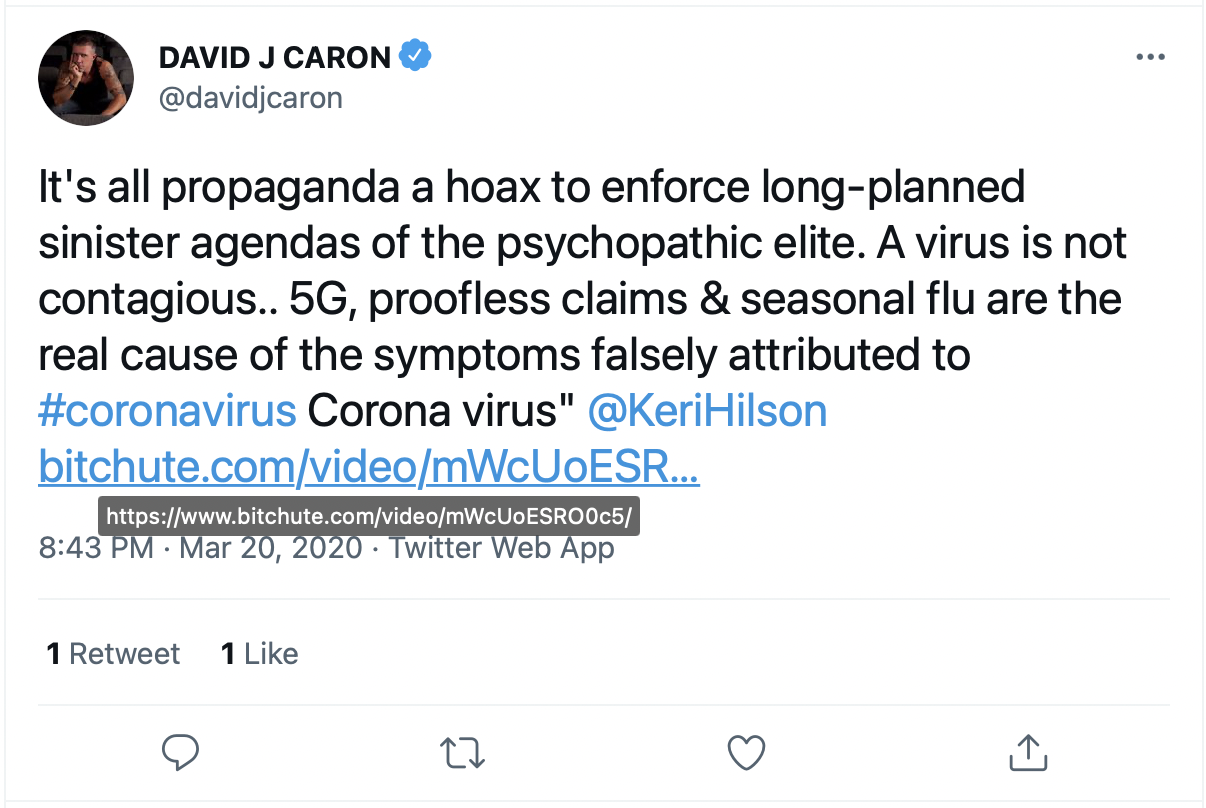
\includegraphics[scale=0.35]{./img/tweets/Capture_2021-06-30_2.png}
   	 %\end{multicols}
	%\begin{multicols}{1} 
		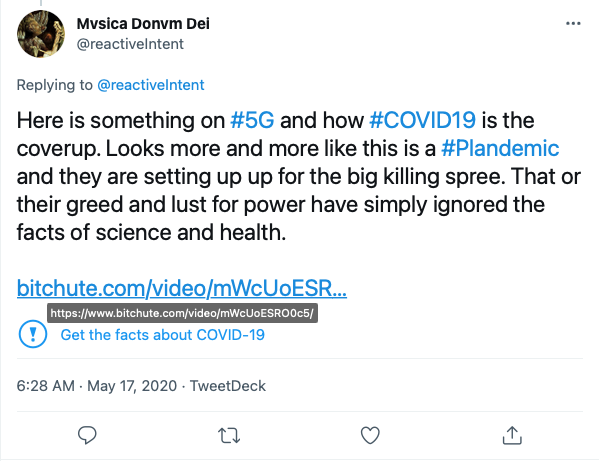
\includegraphics[scale=0.32]{./img/tweets/Capture_2021-06-30.png}
	%\end{multicols}
	\caption{Two tweets sharing the same URL link marked as False by a Fact-Checker, screenshots taken on June 20, 2021. Panel (a): Tweet ID \href{https://twitter.com/davidjcaron/status/1241088065462026242}{1241088065462026242} without a label. Panel (b): Tweet ID \href{https://twitter.com/reactiveIntent/status/1261876171584745472}{1261876171584745472} containing a label.}
	\label{fig8}
\end{figure}

To the best of our knowledge, when using the Twitter API v2, there is no field which indicates whether a tweet is labeled or not; while the interstitial ``possibly sensitive'' and ``withheld" are both Tweet fields that can be recovered\footnote{See \href{https://developer.twitter.com/en/docs/twitter-api/data-dictionary/object-model/tweet}{https://developer.twitter.com/en/docs/twitter-api/data-dictionary/object-model/tweet}.} from the API. Hence, in order to investigate the presence of labels of all types, we resorted to scrape Twitter data using Minet [5]. This tool was recently enriched upon our request in order to capture whether a tweet contains a label or not, via the {\it minet twitter scrape} command.

\smallskip

In this section, we take a deeper look at how labels and notices are introduced by Twitter, to indicate content which is inaccurate or false. To that end, we gathered a set of $3094$ URL links of articles which were marked as $False$ by Science Feedback, a fact-checking organization verifying the credibility of science-related viral information. As a second step, we collected (on June 30, 2021) via Minet Command line tool~\cite{minet} all the tweets that have shared a URL link which belongs to the set of $3094$ links marked as $False$. This data collection resulted in $323$ $938$ tweets, excluding retweets. Only $28$ tweets contained the label { ``Get the facts about COVID-19''}, $5$ tweets contained the label { ``Learn about US 2020 election security efforts''} and only $1$ had the following label {``This claim about election fraud is disputed''}. Furthermore, we noticed that the labeling rule might not be applied uniformly on a given set of tweets sharing the exact same URL link, among the set of collected tweets. More specifically, exactly $657$ tweets had shared a URL link redirecting to a video on Bitchute, entitled ``Important information on coronavirus 5G Kung Flu''. Among those $657$ tweets only $3$ contained the label ``Get the facts about COVID-19'' (see figure \ref{fig8}). This points towards the non-automation of the tweet labelling process and that it might be that these $3$ tweets were the only ones reported by a user. 

\begin{figure}[h]
	\centering
	%\begin{multicols}{1}
		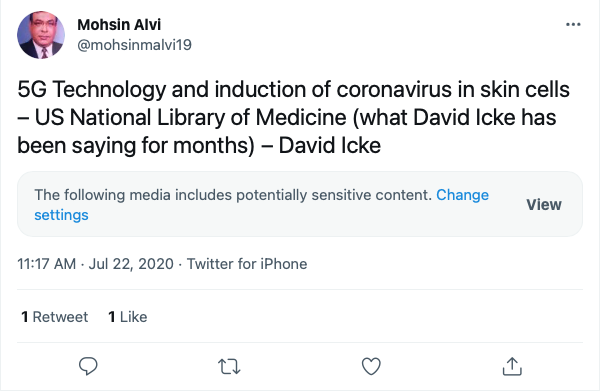
\includegraphics[scale=0.35]{./img/tweets/Capture_2021-07-01_2.png} 
	%\end{multicols}
	%\begin{multicols}{1}
		
\includegraphics[scale=0.35]{./img/tweets/Capture_2021-07-01.png}
	%\end{multicols}
	\caption{Panel (a): Tweet containing a URL link hidden behind an interstitial. Panel (b): when clicking on $view$, to view the content hidden behind the interstitial. Tweet ID \href{https://twitter.com/mohsinmalvi19/status/1285866521533861888}{1285866521533861888}. Screenshots taken on July 1, 2021. }
	\label{fig_notice}
\end{figure}

We further examine the placement of interstitials that indicate a possibly sensitive content. We find that only $2.97\%$ out of $323$ $938$ tweets containing a URL marked as False, have an interstitial ``potentially sensitive content''. {\color{pink}In particular, many tweets speak about COVID19 and do not contain a label to provide users with more context from authoritative sources. Figure \ref{fig_notice} provides an example of a tweet sharing a URL marked as False by a Fact-checker and which contains an interstitial ``potentially sensitive content''.} We find 32 other Tweets, among our set of collected tweets, who share the exact same URL link as in the previous example. Among those 32 Tweets, only 5 tweets had the interstitial ``potentially sensitive content''. Again this points towards the non-automation of the placement of interstitials.\footnote{Notice that the appearance of interstitials may depend on the settings of a user's account and country or language specific regulations. In particular, in the settings of Twitter account, one can deactivate the display of interstitials for {\it sensitive content}, by ticking the box {\it Display media that may contain sensitive content} in the section {\it content you see}. Hence the numbers given are an upper bound of the number of interstitials indicating  possibly sensitive content.} 
{\color{pink} can we have both at the same time (see example facebook)  + dire pour l'exemple get the facts about covid. }
\smallskip

Finally, Twitter Safety account announced in a Tweet\footnote{See Tweet ID : \href{https://twitter.com/TwitterSafety/status/1379515615954620418}{1379515615954620418}} on April 6, 2021 that their team ``will begin deploying automated tools to build on (their) efforts to label tweets that may contain misleading information around COVID-19 vaccinations". 
%we don't know what it means the article xxx which was retracted by the journal and fack-check still appears in xx tweets with no label




\subsection{Youtube}

Youtube may provide an information panel for videos with topics that are prone to misinformation like COVID19, moon landing, and climate change.\footnote{See the section ``Information panel giving topical context'' on Youtube Help, Google accessed on June 28, 2021: \href{https://support.google.com/youtube/answer/9004474?hl=en}{support.google.com/youtube/answer/9004474?hl=en}.} Information panels provide ressources concerning a potentially controversial topic from independent third party partners or authoritative ressources. Youtube states that these panels exist regardless of the point of view expressed in a given video. In addition, these panels are not yet available in all languages and countries. %(“Information panel giving topical context”)

To further study the assignment of information panels to videos, we compiled a list of $171$ Youtube videos, checked by independent fact-checkers\footnote{Is it science Feedback ? if so add.} and marked as containing false or inaccurate information. We collected the information panels, when present, in each video by connecting to a US server and scraping the content of the web page. Four types of information panels were found in the list of visited videos as shown in figure \ref{fig9}:  information about COVID19, Vaccines, Climate change and US elections.

\begin{figure}[h]
	\centering
	%\begin{multicols}{1}
		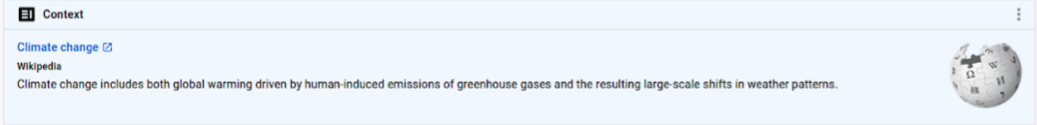
\includegraphics[scale=0.3]{./img/youtube_panels/yt_1.png} 
	%\end{multicols}
	%\begin{multicols}{1}
		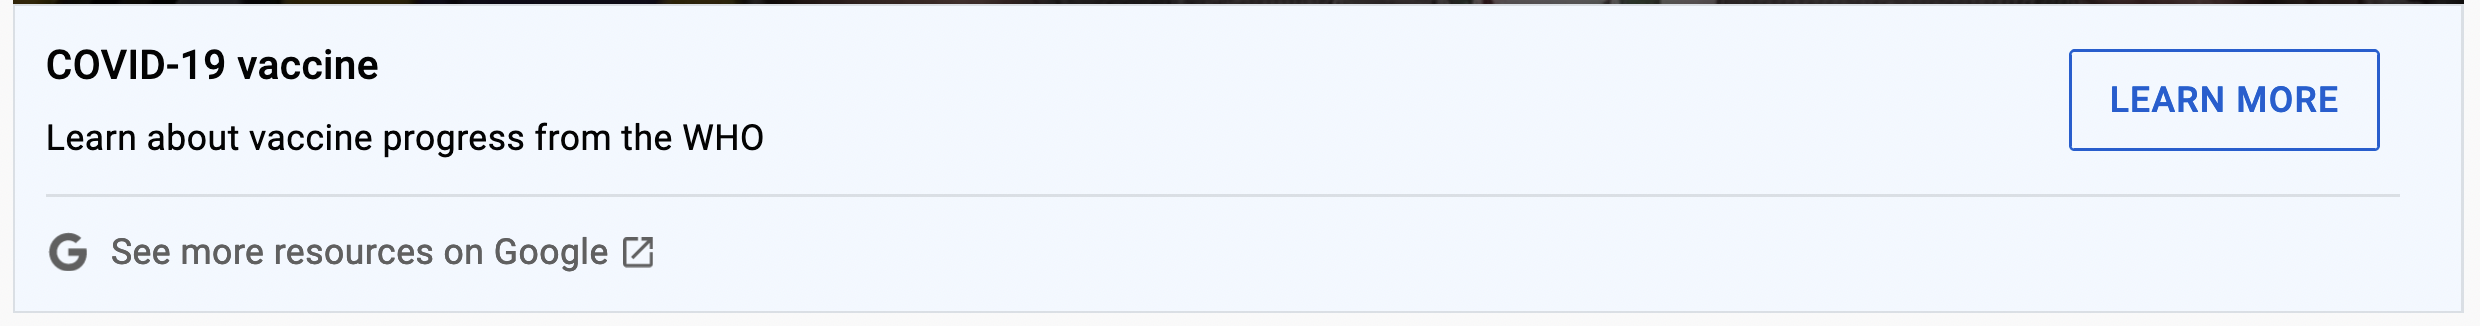
\includegraphics[scale=0.3]{./img/youtube_panels/yt_2.png} 
	%\end{multicols}
	%\begin{multicols}{1}
		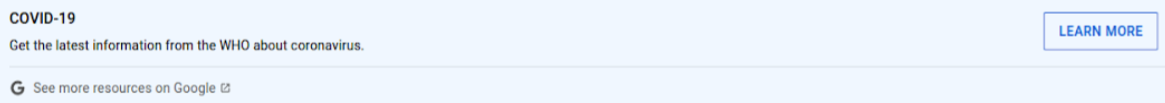
\includegraphics[scale=0.3]{./img/youtube_panels/yt_3.png}
	%\end{multicols}
	%\begin{multicols}{1}
		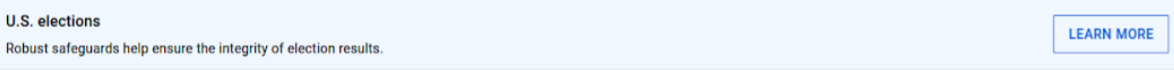
\includegraphics[scale=0.3]{./img/youtube_panels/yt_4.png} 
	%\end{multicols}
	\caption{Examples of YouTube information panels displayed under some videos.}
	\label{fig9}
\end{figure}

We classified the list of Youtube videos by topic based on its content as shown in table \ref{tab2}. We recorded the number of videos containing an information panel within each category. For COVID19 and vaccine related videos more than half of the videos contained an information panel. Nevertheless, we noticed that duplicates of the same Youtube video can get uploaded under different video titles and that the information panel appears under the some duplicates, but not for all. In addition, we noticed for COVID19 related videos, when the video title did not include keywords like (Testing, Pandemic, COVID, coronavirus), the video might not contain a panel associated with it, and in some cases when the video title contains variations of word COVID like (C.O.V.I.D or Cv19) it wouldn’t include a panel either. Therefore, we suspect that youtube is automatically adding panels to the videos based on the video title and not the content of the video.

\smallskip

For climate change we found that most of the videos (13 out of 18) did not display an information panel. Lastly, no information panels were found in the general health category set, that included videos that were not related to COVID19 but contained misinformation concerning cures for cancer, abortion, and viruses. Therefore, it is likely that Youtube add information panels below videos concerning controversial topics that can have misleading information like the climate change, COVID19, flat earth and vaccine. 
%drop last colum
%add % in a second line
\begin{table}[] 
\begin{tabular}{|c|c|c|c|c|}
\hline
Category       & \begin{tabular}[c]{@{}c@{}}Number of Youtube videos {\bf with} an \\ information panel\end{tabular} & \begin{tabular}[c]{@{}c@{}}Number of Youtube videos {\bf without} an \\ information panel\end{tabular}    \\ \hline
\begin{tabular}[c]{@{}c@{}} General Health \end{tabular} & \begin{tabular}[c]{@{}c@{}} 0  \\ (0\%) \end{tabular}  & \begin{tabular}[c]{@{}c@{}} 11 \\ (100\%) \end{tabular}         \\ \hline
Vaccine        & \begin{tabular}[c]{@{}c@{}} 21     \\ (75\%) \end{tabular}   & \begin{tabular}[c]{@{}c@{}}  7 \\ (25\%)  \end{tabular}     \\ \hline
COVID19     & \begin{tabular}[c]{@{}c@{}} 73 \\ (63\%) \end{tabular}  & \begin{tabular}[c]{@{}c@{}} 43  \\ (37\%) \end{tabular}     \\ \hline
\begin{tabular}[c]{@{}c@{}}  Climate change \end{tabular} & \begin{tabular}[c]{@{}c@{}} 5 \\ (28\%) \end{tabular}  & \begin{tabular}[c]{@{}c@{}} 13 \\ (72\%) \end{tabular}   \\ \hline
\end{tabular}
\caption{}
\label{tab2}
\end{table}





%\subsection{Blocking links}

%Another measure that mainstream social media platforms can apply is to prevent users from sharing specific types of content, in this example URLs coming from a specific domain name.


%\subsubsection{Twitter}

%\href{https://help.twitter.com/en/safety-and-security/phishing-spam-and-malware-links}{link}


\section{Reducing the visibility}

Mainstream Social Media platforms can reduce the visibility of the content created or shared by specific users, whenever they violate the platforms' rules. The implementation of this policy varies across platforms and is not easy to verify ex-post. In what follows we provide means to verify this policy on Twitter and Facebook. 
 

\subsection{Facebook}


One of Facebook’s measures to regulate misinformation is to reduce the spread of misleading content through their ranking system. Facebook ranks each post and/or ad by assigning to it a relevancy score, where a high score leads to a high likelihood of the post and/or the ad to appear on a user's newsfeed. Doing so, Facebook can make a post or a whole account less visible by decreasing the relevancy score of its content; this is precisely the $reduce$ measure.\footnote{Lyons, T. (2018, May 22). The three-part recipe for cleaning up your news feed. Facebook Newsroom. \href{https://about.fb.com/news/2018/05/inside-feed-reduce-remove-inform/}{about.fb.com/news/2018/05/inside-feed-reduce-remove-inform/}.} This measure can be verified by looking at the number of views (reach) of a post, but this metric is not available via the APIs used to access Facebook data: CrowdTangle or Buzzsumo. Hence we can indirectly investigate the $reduce$ measure by looking at the engagement metrics (likes, comments, shares) related to a given post; which are available on CrowdTangle and Buzzsumo. If a post reaches less users because it has a lower ranking, then it is less likely to receive likes, comments and shares, relative to a post with a higher ranking. 

%phrase pas accès au reach, mais seulement les engagement metrics
% Owned by Alex Jones, Infowars is usually described as a misinformation website: it is on the Wikimedia global spam blacklist\footnote{See \href{https://meta.wikimedia.org/wiki/Spam\_blacklist}{meta.wikimedia.org/wiki/Spam\_blacklist}.},
%CrowdTangle and Buzzsumo provide access to the interaction metrics on content (engagement), but not to the number of views (or reach), therefore we can only verify the {\it reduce} measure indirectly through a decrease in engagement. If Facebook was reducing the reach of a content via a lower ranking, we would expect the content to be less likely to receive likes, comments and shares, relative to a post with a higher ranking.

\smallskip

To illustrate, we investigate the case of the website $Infowars$. This website appears in the Misinformation Directory of FactCheck.org, among other websites who have posted deceptive content\footnote{See \href{https://www.factcheck.org/2017/07/websites-post-fake-satirical-stories/}{https://www.factcheck.org/2017/07/websites-post-fake-satirical-stories/}.}. Furthermore, the factual reporting of $Infowars$ has been rated {\it very low} by the Media Bias / Fact Check resource of Iffy.news.\footnote{See the Iffy.news page: \href{https://mediabiasfactcheck.com/infowars-alex-jones/}{https://mediabiasfactcheck.com/infowars-alex-jones/}.} 

\begin{figure}[h]
	\centering
	
	%\begin{multicols}{1}
		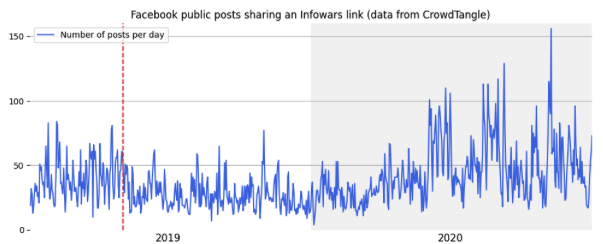
\includegraphics[scale=0.3]{./img/infowars/fb_infowars_1.png}
	%\end{multicols}
	%\begin{multicols}{1}
		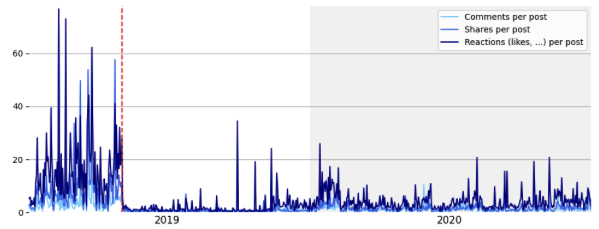
\includegraphics[scale=0.3]{./img/infowars/fb_infowars_2.png} 
	%\end{multicols}
	
	\caption{Public Facebook posts sharing an Infowars link in $2019$ and $2020$ collected from the CrowdTangle API. The red line marks the date of May $2$, 2019, when Facebook has announced the ban regarding Infowars. (Top panel) Number of daily posts. (Bottom panel) Engagement metrics: average number of reactions, shares and comments per post. }
	\label{infowars1}
\end{figure}

On May 2, 2019, Facebook announced they would prohibit users from sharing Infowars content unless, they are explicitly condemning the material.\footnote{See \href{https://www.wired.com/story/facebook-bans-alex-jones-extremists/}{https://www.wired.com/story/facebook-bans-alex-jones-extremists/} and \href{https://about.fb.com/news/2018/08/enforcing-our-community-standards/}{about.fb.com/news/2018/08/enforcing-our-community-standards/}.} To verify the measure, we used the ``/posts/search'' endpoint\footnote{see the documentation for more details: \href{https://github.com/CrowdTangle/API/wiki/Search}{github.com/CrowdTangle/API/wiki/Search}.} of the CrowdTangle API, to collect $37$ $242$ Facebook public posts that had shared a URL link containing ``infowars.com'', published between January $1$, $2019$ and December $31$, $2020$.\footnote{We found in the collected data some Facebook posts that did not directly share an Infowars link (but rather a YouTube or Facebook video containing an Infowars link in its description), thus we excluded such posts from our data to keep only the $27$ $721$ posts directly sharing an Infowars link.} The command used can be found in the following Github repository: \href{https://github.com/medialab/truth-and-trust-online-2021/blob/master/code/collect_facebook_crowdtangle_infowars_data.sh}{link}. The number of public posts sharing an $Infowars$ link remained globally stable throughout $2019$ (see figure \ref{infowars1} top panel). Thus the measure announced by Facebook doesn't seem to have prevented users from sharing an $Infowars$ link. Nevertheless, a clear drop in engagement was observed on May 2, 2019 (see figure \ref{infowars1} bottom panel). The number of reactions, shares and comments per post have decreased respectively  by $-94\%$,  $-96\%$ and $-93\%$  when comparing the two months before and after May 2, 2019. This suggests the measure taken by Facebook in May $2019$, is not a ban per se, but rather a $reduce$ measure. This is because users could still post $Infowars$ links, but these posts generated less engagement. It should be noted that the engagement metrics increased again by the end of $2019$ / beginning of $2020$, suggesting that the $reduce$ measure may have been lifted a few months after its implementation.

\begin{figure}[h]
	\centering
	
	%\begin{multicols}{1}
		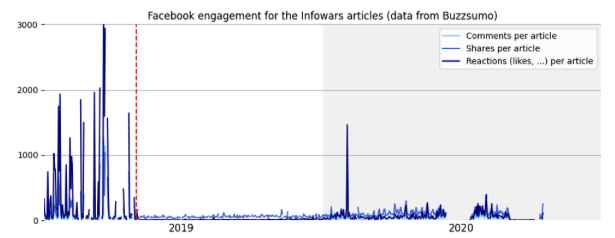
\includegraphics[scale=0.35]{./img/infowars/fb_infowars_3.png}
	%\end{multicols}

	\caption{Facebook engagement metrics (average number of reactions, shares and comments per article) for the Infowars articles published in $2019-2020$ and gathered from the Buzzsumo API. The red line marks the date of May $2$, $2019$, when Facebook has announced the ban regarding Infowars.}
	\label{infowars2}
\end{figure}

As CrowdTangle is tracking posts only from certain public groups and pages, we also used the ``/search/articles'' endpoint of the Buzzsumo API, to gather a richer Facebook dataset. We collected the engagement data for the $14$ $232$ articles crawled by Buzzsumo from the $Infowars$ website between January $1$, $2019$ and December $31$, $2020$.  \footnote{The command can be found: \href{https://github.com/medialab/truth-and-trust-online-2021/blob/master/code/collect\_facebook\_buzzsumo\_infowars\_data.py}{here}.} We observe that the articles published after May $2$, $2019$ received less Facebook engagement than the ones published before (see figure \ref{infowars2}), with a percentage change of -$97\%$ for the reactions, -$59\%$ for the shares and -$97\%$ for the comments. An increase in engagement was also observed in $2020$. It reinforces the hypothesis that Facebook reduced the reach of posts sharing Infowars links only during a few months in $2019$.

We found irregularities in the number of Infowars articles collected from Buzzsumo. While Infowars usually publishes around 800 articles per month, only 53 articles were collected between June 11 to July 11, 2020\footnote{In Figure \ref{infowars2} the engagement metrics were only shown for days in which at least 5 Infowars articles were collected from Buzzsumo, to ensure reliable results.}. A temporary crawling problem coming from Buzzsumo may have caused this lack of data. Because no database is perfect, we would like to highlight the importance of cross-checking information between different sources when possible.

\subsubsection{Facebook}

The Beauty of life (\href{https://thebl.com/}{thebl.com/}) is a US-based media company that shares pro-Trump views and conspiracy theories such as QAnon.\footnote{ See \href{https://en.wikipedia.org/wiki/The\_Epoch\_Times\#Removal\_of\_The\_BL\_(The\_Beauty\_of\_Life)\_from\_Facebook}{wikipedia article}.} Facebook has announced on December $20$, $2019$ that ``The BL is now banned from Facebook'' for coordinated inauthentic behavior\footnote{\href{https://about.fb.com/news/2019/12/removing-coordinated-inauthentic-behavior-from-georgia-vietnam-and-the-us/}{https://about.fb.com/news/2019/12/removing-coordinated-inauthentic-behavior-from-georgia-vietnam-and-the-us/}.}, which includes using fake accounts that misrepresent one's identity or using methods to artificially boost the popularity of content. Coordinated inauthentic behavior is a distinct phenomenon from disinformation according to Facebook, as ``most of the content shared by coordinated manipulation campaigns isn’t probably false”.\footnote{See: \href{https://about.fb.com/news/2019/10/inauthentic-behavior-policy-update/}{https://about.fb.com/news/2019/10/inauthentic-behavior-policy-update/}.} Nevertheless, for the case of the Beauty of Life, both misinformation and coordinated inauthentic behavior were attested, according to the fact-checking organization Snopes which had reported about The BL’s activity to Facebook and other various public articles\footnote{\href{ https://www.snopes.com/news/2019/11/12/bl-fake-profiles/}{https://www.snopes.com/news/2019/11/12/bl-fake-profiles/}, \href{https://www.snopes.com/news/2019/11/12/bl-fake-profiles/}{https://www.snopes.com/news/2019/11/12/bl-fake-profiles/}, \href{https://www.snopes.com/news/2019/12/13/facebook-bl-cib/}{https://www.snopes.com/news/2019/12/13/facebook-bl-cib/}}.

\begin{figure}[h]
	\centering
	
	%\begin{multicols}{1}
		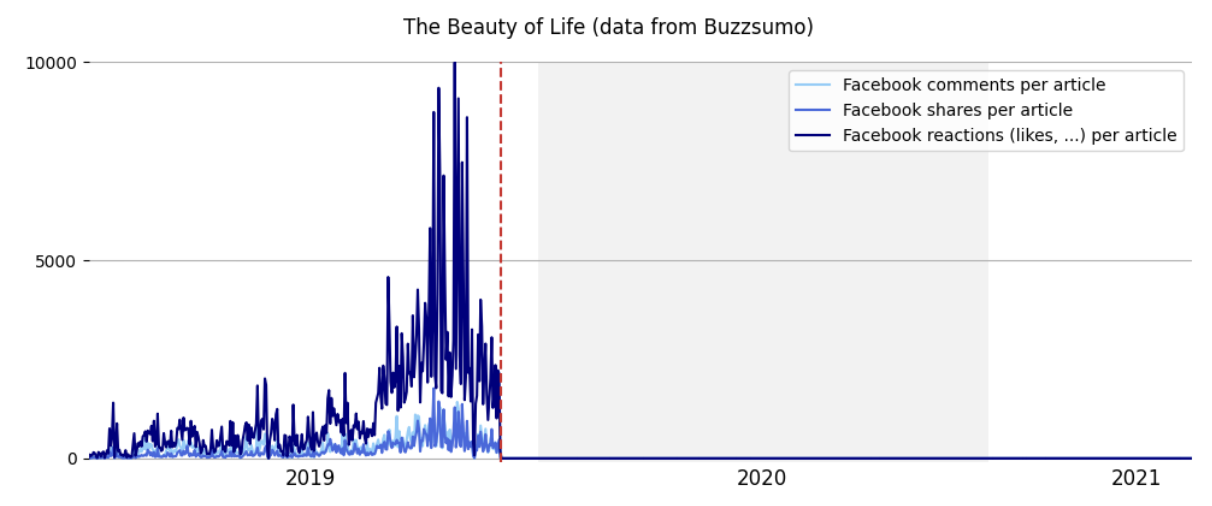
\includegraphics[scale=0.3]{./img/beautyoflife/fb_bl_1.png}
	%\end{multicols}
	%\begin{multicols}{1}
		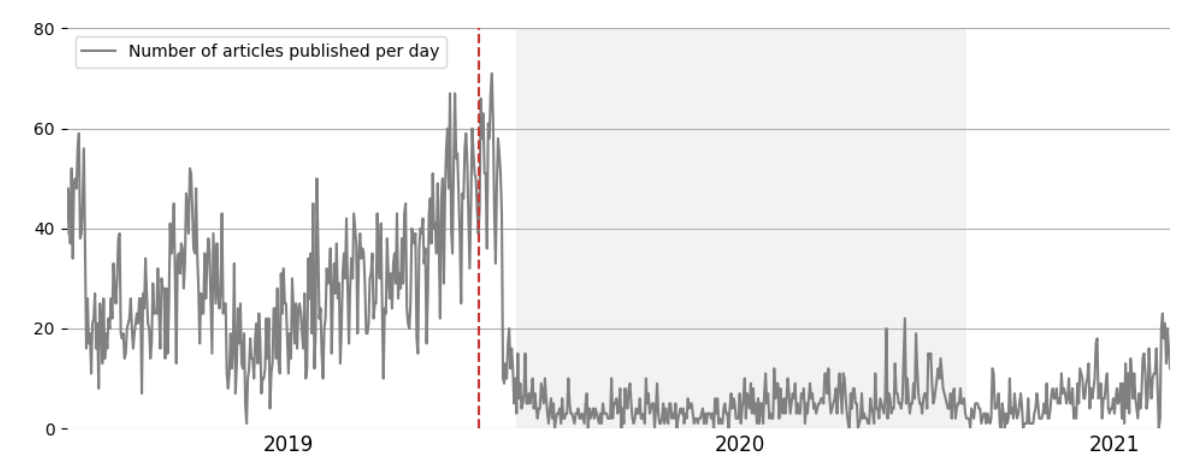
\includegraphics[scale=0.3]{./img/beautyoflife/fb_bl_2.png} 
	%\end{multicols}
	
	\caption{Articles from The Beauty of Life website (thebl.com) published between January 1, 2019 and June 15, 2021 and gathered from the Buzzsumo API. (Top) Facebook engagement metrics (average number of reactions, shares and comments per article). (Bottom) Number of articles published per day. The red line marks the date of December 1, 2019. }
	\label{fb_bl}
\end{figure}
%BuzzSumo is a commercial content database that tracks the volume of user interactions with internet content on Facebook, Twitter, and other social media platforms. 

To verify Facebook’s ban of The BL domain name, we first tested whether we could post a Facebook message containing a url from thebl.com. This turned out to be impossible. But such manual verification cannot inform us whether the ban applies indeed to all Facebook users and accounts (as we used only our own personal accounts), nor when it has started. To further investigate this policy, we collected data from the Buzzsumo API\footnote{BuzzSumo is a commercial content database that tracks the volume of user interactions with internet content on Facebook, Twitter, and other social media platforms.}. We used the ``/search/articles'' endpoint to collect the engagement metrics of the $13$ $634$ articles crawled from the $thebl.com$ website between January $1$, $2019$ and June $15$, $2021$.\footnote{The command can be found in the following Github repository: \href{https://github.com/medialab/truth-and-trust-online-2021/blob/master/code/collect\_facebook\_buzzsumo\_thebl\_data.py}{https://github.com/medialab/truth-and-trust-online-2021/blob/master/code/collect\_facebook\_buzzsumo\_thebl\_data.py}.}

The number of Facebook reactions, shares and comments dropped to zero for TheBL’s articles published after December $1$, $2019$ (see figure \ref{fb_bl} top panel), indicating the start of the ban. We can note that although the ban was communicated in an article\footnote{See \href{https://about.fb.com/news/2019/12/removing-coordinated-inauthentic-behavior-from-georgia-vietnam-and-the-us}{https://about.fb.com/news/2019/12/removing-coordinated-inauthentic-behavior-from-georgia-vietnam-and-the-us}.} published on December $20$, $2019$, it seems to have actually started on December $1$, $2019$.

The communication around the ban appeared to have discouraged The Beauty of Life to proceed with their activity. Indeed the number of articles they published daily was around $50$ until December $20$, $2019$, when it decreased drastically to reach around $5$ to $10$ articles published per day (see figure \ref{fb_bl} bottom panel). Using Buzzsumo data, we ascertained that links from thebl.com were not shared on Facebook anymore. The ban started on December $1$, $2019$, and appeared to be still enforced in June 2021.

\subsection{Twitter} 

Twitter can take action against a tweet which violates the Twitter rules\footnote{See the paragraph {\it Limiting Tweet visibility}: \href{https://help.twitter.com/en/rules-and-policies/enforcement-options}{https://help.twitter.com/en/rules-and-policies/enforcement-options}.}, by limiting its visibility on users' timelines and in search results. To illustrate we provide an example for the website $globalresearch.ca$, which has several failed fact-checks according to \href{https://iffy.news}{iffy.news} - a website which provides a database of websites with low factual reporting levels.\footnote{For $globalresearch.ca$ see \href{https://mediabiasfactcheck.com/global-research/}{https://mediabiasfactcheck.com/global-research/}.}

%\smallskip

%To illustrate we provide two examples linked to the Twitter accounts of the websites $globalresearch.ca$ and $off$-$guardian.org$. Both websites have several failed fact-checks according to \href{https://iffy.news}{iffy.news} - a website which provides a database of websites with low factual reporting levels.\footnote{For $globalresearch.ca$ see \href{https://mediabiasfactcheck.com/global-research/}{https://mediabiasfactcheck.com/global-research/} and for $off-guardian.org$ see \href{https://mediabiasfactcheck.com/offguardian/}{https://mediabiasfactcheck.com/offguardian/}.  }
\begin{figure}[h]
	\centering
		%\begin{multicols}{1}	
			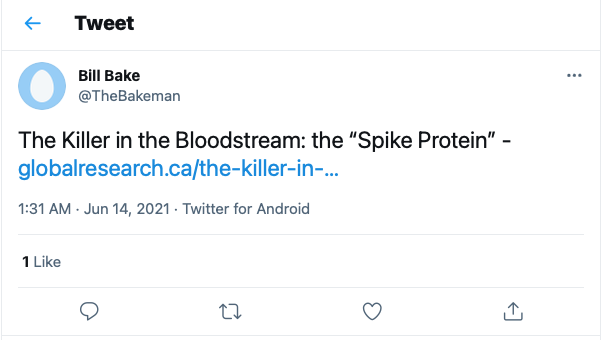
\includegraphics[scale=0.32]{./img/globalresearch/tweet.png} 
		%\end{multicols}
		%\begin{multicols}{1}
			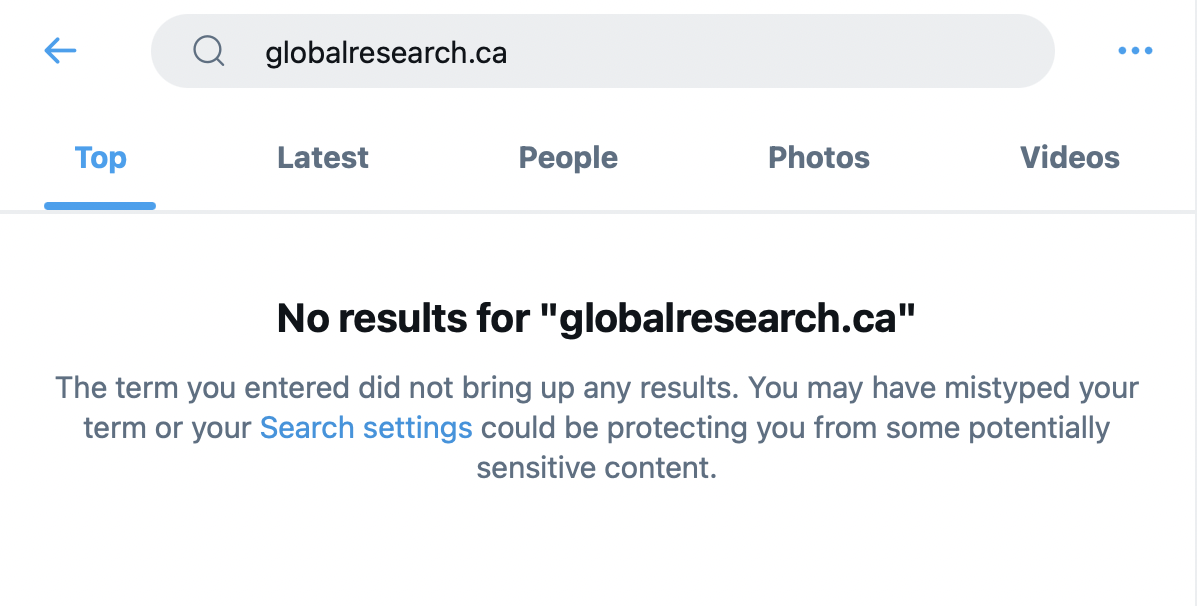
\includegraphics[scale=0.35]{./img/globalresearch_14_06_2021_16pm_UTC.png} 
		%\end{multicols}
		\caption{Screenshots taken on June 14, 2021. Top panel: ? . Bottom panel: screenshot that shows that no results can be found when searching for $globalresearch.ca$.    }
		\label{fig3}
\end{figure}


The website $globalresearch.ca$ is linked to the Twitter account {$@CRG\_CRM$}; which was recently suspended.\footnote{We noticed the message about the account suspension on May 25, 2021. But to the best of our knowledge, no official communication by Twitter has announced the suspension nor the exact date at which it was implemented. Hence the account may have gotten suspended anytime between April 15, 2021 and May 25, 2021 (see the suspension screenshot in panel $(a)$ of figure \ref{fig3}). Furthermore, $globalresearch.ca$ has multiple failed fact-checks, see \href{https://mediabiasfactcheck.com/global-research/}{https://mediabiasfactcheck.com/global-research/} and \href{https://feedback.news/media/AEKA}{https://feedback.news/media/AEKA}.} When a user searches via the twitter search-box for any URL link of this website, no results appear as shown in the screenshot in panel $(b)$ of figure \ref{fig3}, taken on June $14$, $2021$. To further investigate the possible implementation of a reduced visibility measure, we search via the Twitter API for tweets, excluding retweets, containing the query {\it globalresearch.ca} from January $1$, $2021$ until June $10$, $2021$.  As shown in panel (a) in figure \ref{fig4}, we find a strictly positive number of tweets containing the URL link {\it globalresearch.ca} throughout May $2021$ and the first week of June $2021$. Hence, the visibility of tweets containing this URL link has been reduced because users can no longer access tweets containing the URL link {\it globalresearch.ca} via the search box. Nevertheless users are not restrained from posting tweets containing this URL, as shown in the screenshot in panel $(a)$ of figure \ref{fig4bis}, found by taking the tweet ID of one of the collected tweets via the Twitter API. Furthermore, those collected Tweets have strictly positive engagement metrics as shown in panel $(b)$ of figure \ref{fig4}. Hence, the users who tweet articles from the {\it globalresearch.ca} website receive tweet level engagement from their own followers. Finally, when a user attempts to click on the URL link {\it globalresearch.ca} contained in the Tweet, a warning message appears and indicates that the link may be unsafe (see screenshot in panel (b) in figure \ref{fig4bis}). 

The website $globalresearch.ca$ is linked to the Twitter account {$@CRG\_CRM$}; which was recently suspended.\footnote{We noticed the message about the account suspension on May 25, 2021. But to the best of our knowledge, no official communication by Twitter has announced the suspension nor the exact date at which it was implemented. Hence the account may have gotten suspended anytime between April 15, 2021 and May 25, 2021 (see the suspension screenshot in panel $(a)$ of figure \ref{fig3}).} When a user searches via the twitter search-box for any URL link of this website, no results appear as shown in the screenshot in panel $(b)$ of figure \ref{fig3}, taken on June $14$, $2021$. 

\begin{figure}[h]
\centering
	%\begin{multicols}{1}
		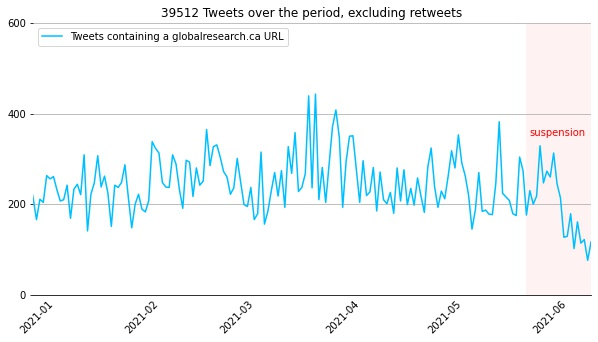
\includegraphics[scale=0.35]{./img/globalresearch/sum_globalresearch.ca_6_months.jpg} 
	%\end{multicols}
	%\begin{multicols}{1}
		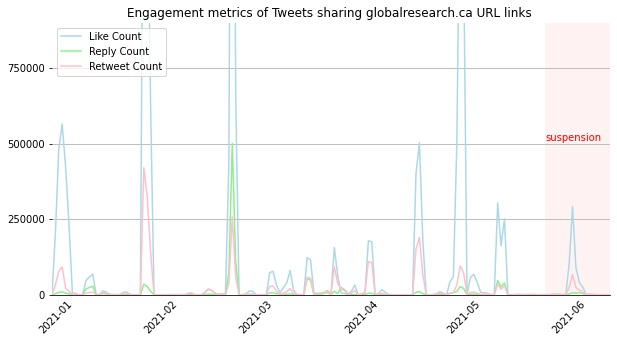
\includegraphics[scale=0.35]{./img/globalresearch/engagement_sum_rolling_1_globalresearch.ca.jpg}
	%\end{multicols}
\caption{Top panel: daily number of Tweets, excluding retweets, containing the query {\it globalresearch.ca} from January $1$, $2021$ until June $10$, $2021$. Bottom panel: engagement metrics of Tweets containing the query {\it globalresearch.ca} from January $1$, $2021$ until June $10$, $2021$. Data collected via the Twitter API v2 on June $16$, 2021.   }
\label{fig4}
\end{figure}

To further investigate the possible implementation of a reduced visibility measure, we search via the Twitter API for tweets, excluding retweets, containing the query {\it globalresearch.ca} from January $1$, $2021$ until June $10$, $2021$.  As shown in panel (a) in figure \ref{fig4}, we find a strictly positive number of tweets containing the URL link {\it globalresearch.ca} throughout May $2021$ and the first week of June $2021$. Hence, the visibility of tweets containing this URL link has been reduced because users can no longer access tweets containing the URL link {\it globalresearch.ca} via the search box. Nevertheless users are not restrained from posting tweets containing this URL, as shown in the screenshot in panel $(a)$ of figure \ref{fig4bis}, found by taking the tweet ID of one of the collected tweets via the Twitter API. Furthermore, those collected Tweets have strictly positive engagement metrics as shown in panel $(b)$ of figure \ref{fig4}. Hence, the users who tweet articles from the {\it globalresearch.ca} website receive tweet level engagement only from their own followers. 

Finally, when a user attempts to click on the URL link {\it globalresearch.ca} contained in the Tweet, a warning message appears and indicates that the link may be unsafe (see screenshot in panel (b) in figure \ref{fig4bis}). 


\begin{figure}[h]
\centering	
	%\begin{multicols}{1}
		%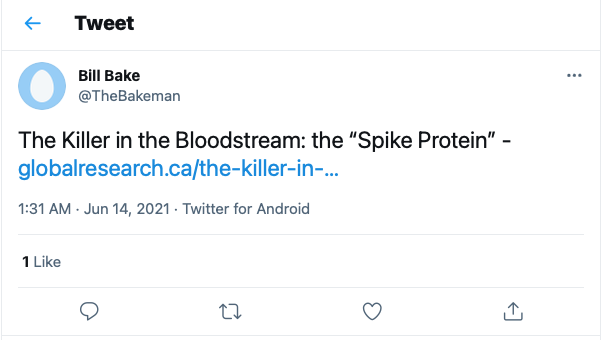
\includegraphics[scale=0.35]{./img/globalresearch/tweet.png} 
	%\end{multicols}
	%\begin{multicols}{1}
		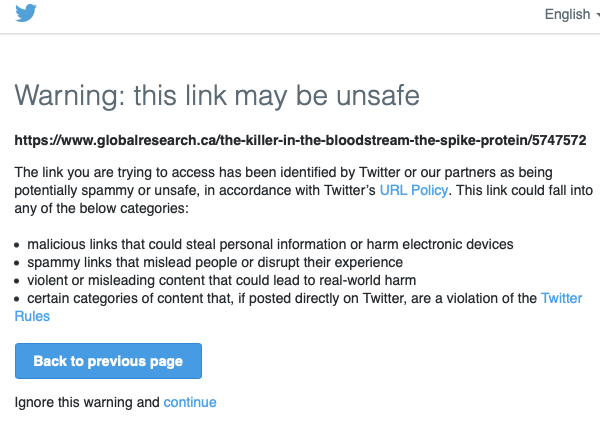
\includegraphics[scale=0.35]{./img/globalresearch/warning.png}
	%\end{multicols}
\caption{}
\label{fig4bis}
\end{figure}


%We provide a second example with the website $off$-$guardian.org$. Unlike the previous example, the Twitter account linked to this website is not currently\footnote{The account can be accessed via the Twitter handle $@OffGuardian0$ and we verified on June 13, 2021 that the account is not suspended.} suspended. 

%off guardian: people put space before .com but they can still share off-guardian links  (test Héloïse). why do they do that? 
%warning page before accessing the website - always 
%twitter API doesn't return the tweets tweeted by off-guardian themselves dating back to 2015
%twitter API returns both tweets with . org and .org: 320 tweets from 2017-01-15 until 2021-06-11. But off-guardian themselves posted one of their own links on June 16 2021. 
%minet returns almost nothing : 43 tweets 
% the tweets created by Off-Guardian: don't come up in the search box. Unlike nytimes.com their articles do appear in the search box , published by themselves! 
% Heloise's tweet June 15 doesn't come up in the API ! 
% people use variants with * and dot , so that they can find tweets speaking about those domains

\subsection{Youtube}

{\color{pink} What about something about recommendations ? authoritative content  }



\section{Discussion}


{ \color{pink} 
Sporadic points for the discussion, no structure yet. 

\begin{itemize}

	\item For a previous research project\footnote{reference?}, we searched on CrowdTangle for public accounts sharing specific content associated with misinformation in November $2020$, and selected $94$ Facebook pages corresponding to our criteria. We then tried to collect these pages' posts in January $2021$, and discovered that $11$ pages could not be found anymore. This highlights an important issue when studying misinformation trends on Facebook: some data disappears from the CrowdTangle API as accounts are deleted or changed to {\it private}. 

	\item To facilitate the verification in the policy applications, we would generally recommend for the platforms to be more transparent. But too much transparency on how the regulation policies are exactly implemented can actually backfire. For example YouTube is certainly applying an 'information' banner on all videos mentioning Covid and related terms in their title. Misinformation accounts are trying to avoid the official banners by using terms as 'C.O.V.I.D' or 'C O V I D'. If YouTube was totally transparent on that matter and published the list of 'dangerous' words that leads to an information banner, this list would of course help us to understand YouTube's policies but it would also help the misinformation actors to escape the regulation. There is thus a balance between communicating enough so the public can know precisely how the platforms are regulating their content, but without giving too much information that would allow the policies to be bypassed.

	\item There are other ways to collect data from platforms, and besides Buzzsumo, other API are also aggregating data from multiple social platforms. For example Newsguard, blablabla... In this tweet, we can see the interface of XXX being used in this study from a data journalist: \href{https://twitter.com/Shayan86/status/1394742784683298818/photo/2}{ex}

	\item Recommendation: inform about sources, example inform users that this user shared x failed fact-checks. 

	\item Make point about ``recycling" existing policies (e.g. to tackle terrorism) and apply it to misinformation+

	\item Make point about the communication of platforms for their policy: 4R of Youtube, RRI of Facebook, 

	\item Make point that platforms when they take actions regarding misinformation, they rarely cite misinformation as the reason. E.g. beauty of life, coordinated inauthentic behavior. 

\href{https://misinforeview.hks.harvard.edu/article/tackling-misinformation-what-researchers-could-do-with-social-media-data/}{https://misinforeview.hks.harvard.edu/article/tackling-misinformation-what-researchers-could-do-with-social-media-data/}

	\item After a channel gets suspended or a video is deleted the data related to them is removed from the youtube API. This is a problem that affected the study to investigate the suspension reasons or the removal. For instance, the original list of videos from table 1 had more than 200 videos available in March 2021, however, by June 2021 30 videos got deleted from youtube because they contain content that is against the youtube guidelines and their data got removed from the API. 
	
	\item User side: psychological effects (Pennycook, etc.), multi-platforms, indirect effects, strategies... 
	
	\item business model 
	
	\item Pas accès au ``reach" !  ranking not available. Fb nous a donné certaines données (les données Condor) et dedans on a le nombre de clicks par exemple
	
	\item ``All four Pages have been unpublished for repeated violations of Community Standards and accumulating too many strikes. While much of the discussion around Infowars has been related to false news, which is a serious issue that we are working to address by demoting links marked wrong by fact checkers and suggesting additional content, none of the violations that spurred today’s removals were related to this." \href{https://about.fb.com/news/2018/08/enforcing-our-community-standards/}{Newsroom}.
	\item Researchers should be able to access the data of deleted accounts on the main platforms.

	\item Currently the flag or notice banners data is not present in the platforms’ API datasource, and this prevents researchers and journalists from easily investigating that matter. They have to use or build a scraper to access the data.

	\item Lack of transparency in the platforms’ communication that makes their policies harder to verify.

	\item Finally, we found irregularities in the number of Infowars articles collected from Buzzsumo. While Infowars usually publishes $20$ to $30$ articles per day, only $53$ articles were collected in the $31$-day period between June $11$ to July $11$, 2020. A temporary crawling problem coming from Buzzsumo may have caused this lack of data. Because no database is perfect, we would like to highlight the importance of cross-checking information between different sources when possible. 
\end{itemize}
}


 

\bibliography{proj1}{}
\bibliographystyle{plain}

\newpage 

\section{Appendix}

\subsection{Quick access to community guidelines and policies} \label{links}

\begin{landscape}

\begin{table*}[h]
\begin{tabular}{|c|c|c|}
\hline
\multirow{3}{*}{Rules}                     & 
\includegraphics[scale=0.05]{./img/fb_logo.png} & \href{https://www.facebook.com/communitystandards/recentupdates/}{facebook.com/communitystandards/recentupdates/}                         \\ \cline{2-3} 
                                           & 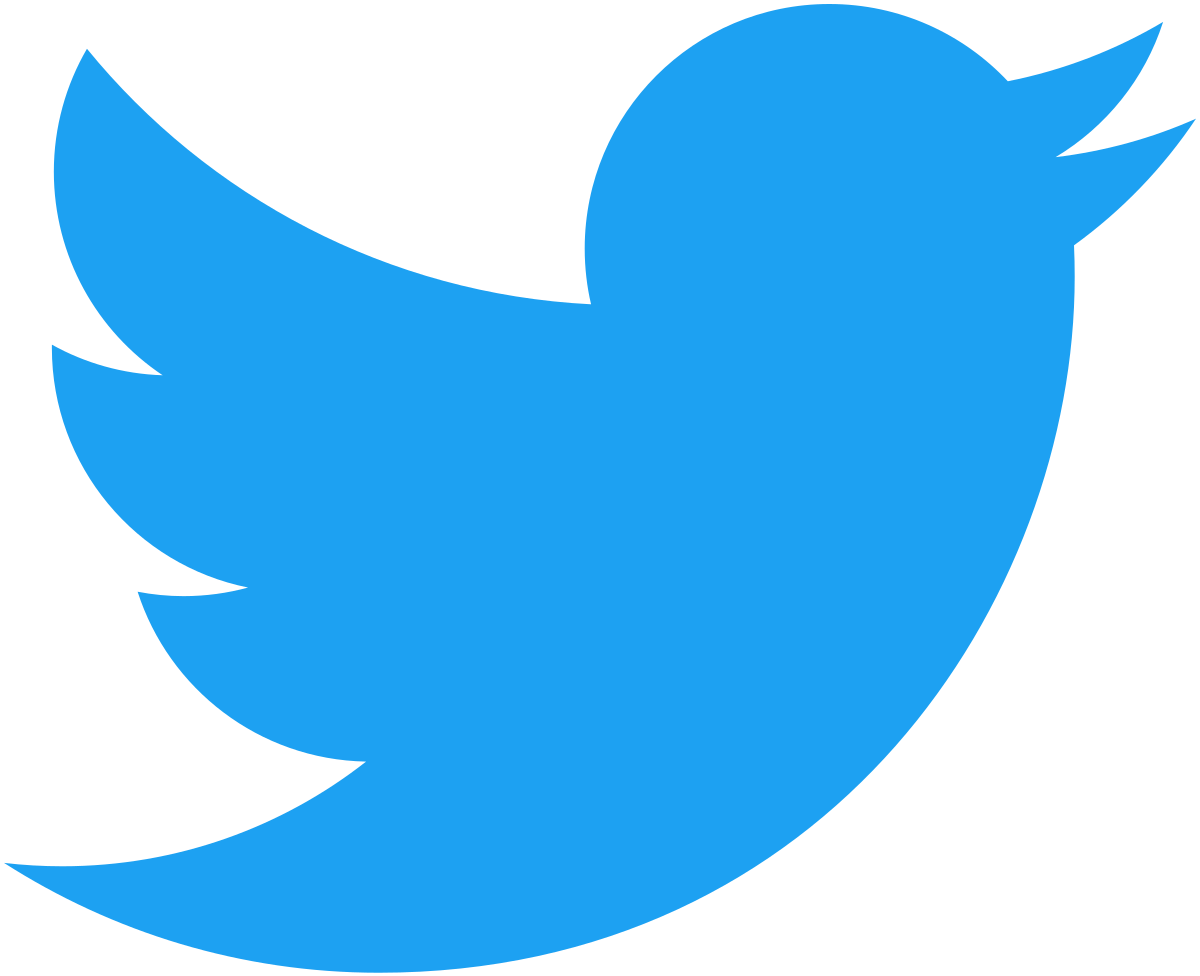
\includegraphics[scale=0.007]{./img/tw_logo.png}   & \href{https://help.twitter.com/en/rules-and-policies/twitter-rules}{help.twitter.com/en/rules-and-policies/twitter-rules}                       \\ \cline{2-3} 
                                           & 
\includegraphics[scale=0.03]{./img/yt_logo.png}  & \href{https://www.youtube.com/intl/en\_us/howyoutubeworks/policies/community-guidelines/}{youtube.com/intl/en\_us/howyoutubeworks/policies/community-guidelines/} \\ \hline
\multirow{3}{*}{\begin{tabular}[c]{@{}cl@{}}  Rules \\ enforcement \end{tabular}}         & 
\includegraphics[scale=0.05]{./img/fb_logo.png}  & \href{https://transparency.fb.com/data/community-standards-enforcement/}{transparency.fb.com/data/community-standards-enforcement/}                 \\ \cline{2-3} 
                                           & 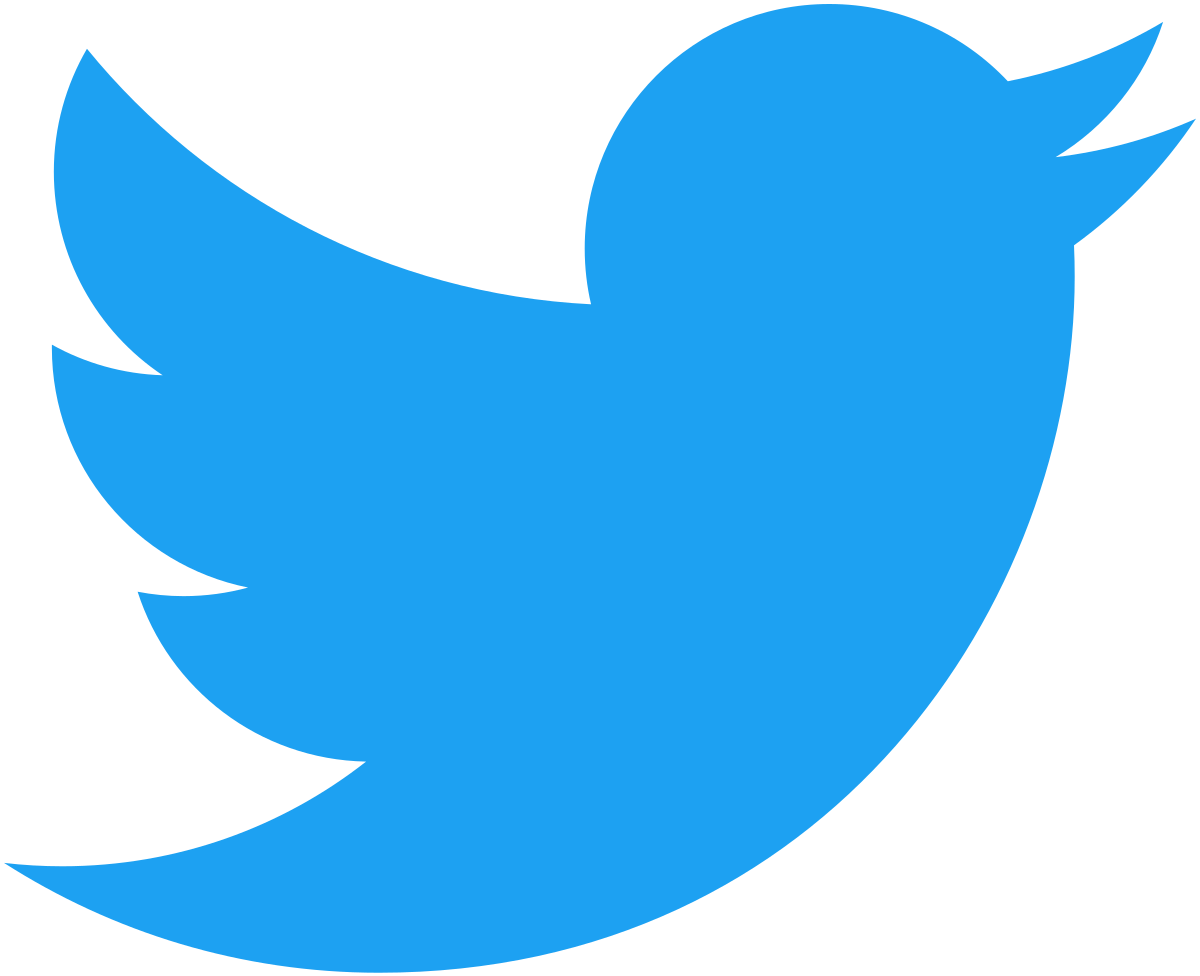
\includegraphics[scale=0.007]{./img/tw_logo.png}   & \href{https://transparency.twitter.com/en/reports/rules-enforcement.html}{transparency.twitter.com/en/reports/rules-enforcement.html}                \\ \cline{2-3} 
                                           & 
\includegraphics[scale=0.03]{./img/yt_logo.png}  & \href{https://transparencyreport.google.com/youtube-policy/}{transparencyreport.google.com/youtube-policy/}                              \\ \hline
\multirow{3}{*}{\begin{tabular}[c]{@{}cl@{}}  Transparency \\ center \end{tabular}}       & 
\includegraphics[scale=0.05]{./img/fb_logo.png} & https://transparency.fb.com/data/                                                  \\ \cline{2-3} 
                                           & 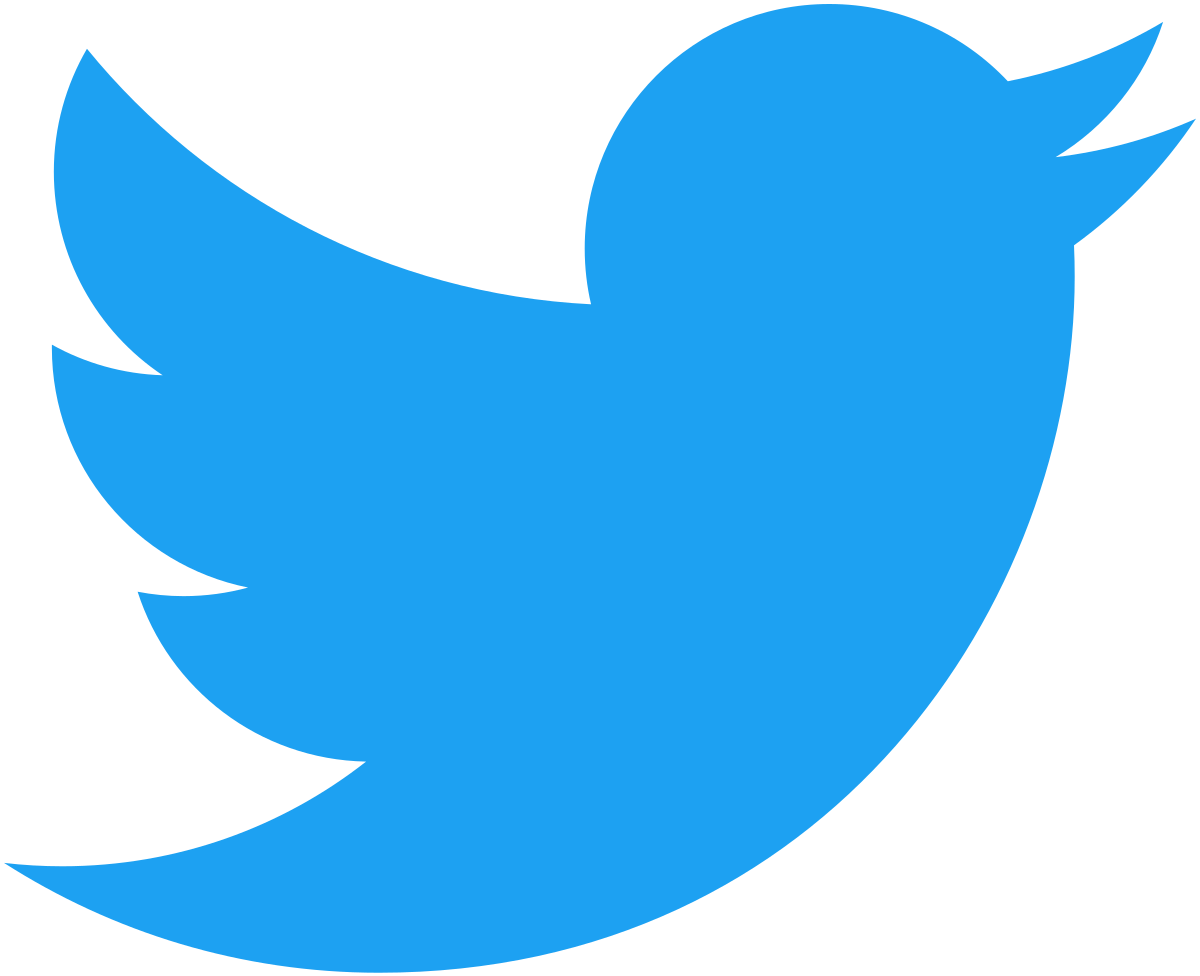
\includegraphics[scale=0.007]{./img/tw_logo.png}   & \href{https://transparency.twitter.com/en/reports.html}{transparency.twitter.com/en/reports.html}                                  \\ \cline{2-3} 
                                           & 
\includegraphics[scale=0.03]{./img/yt_logo.png}  & \href{https://transparencyreport.google.com/?hl=en}{transparencyreport.google.com/?hl=en}                                      \\ \hline
\multirow{3}{*}{\begin{tabular}[c]{@{}cl@{}}  Policy \\ regarding \\  Covid-19 \end{tabular}} & 
\includegraphics[scale=0.05]{./img/fb_logo.png} & https://www.facebook.com/help/230764881494641/                                     \\ \cline{2-3} 
                                           & 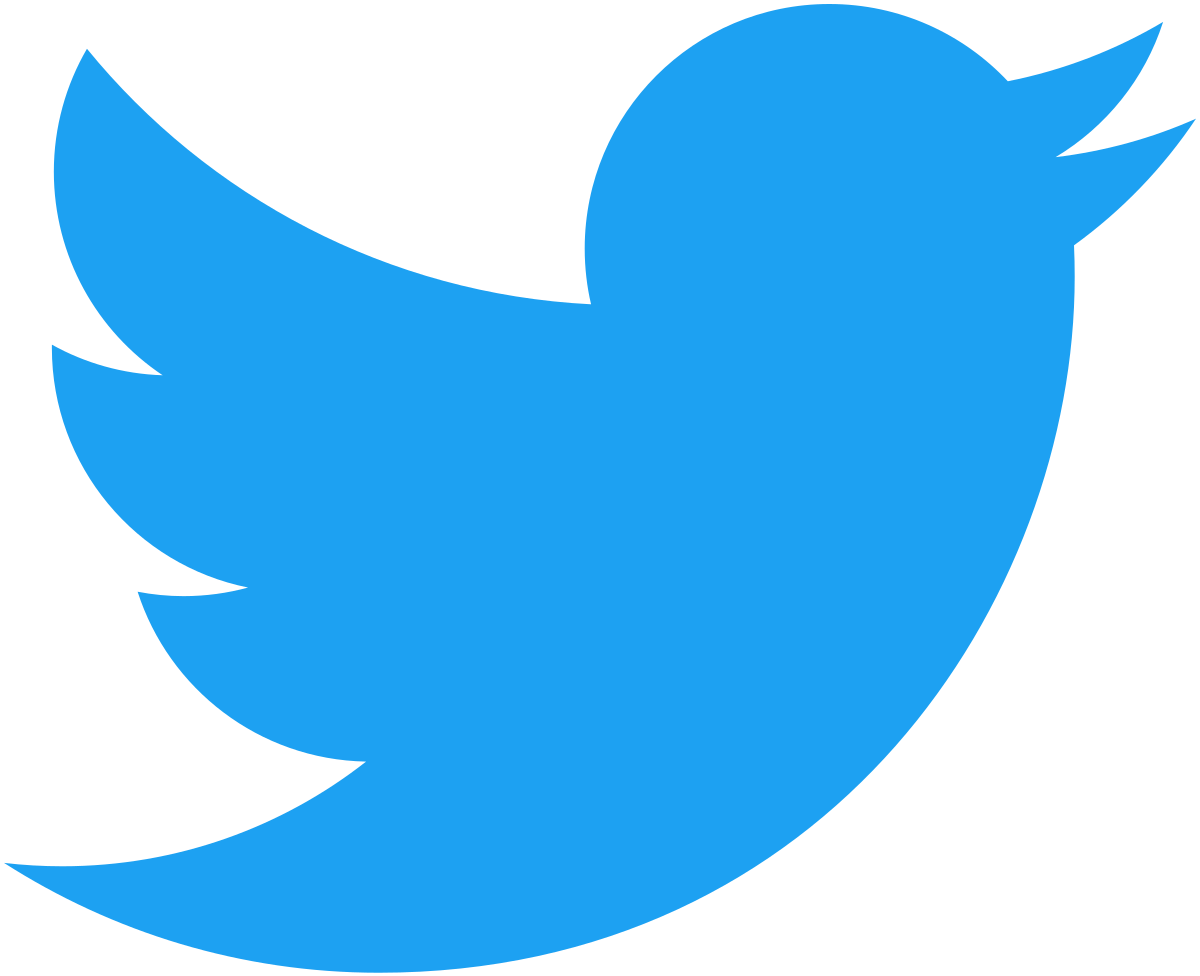
\includegraphics[scale=0.007]{./img/tw_logo.png}   & \begin{tabular}[c]{@{}cl@{}} \href{https://help.twitter.com/en/rules-and-policies/medical-misinformation-policy}{help.twitter.com/en/rules-and-policies/medical-misinformation-policy} \\  \href{https://blog.twitter.com/en\_us/topics/company/2021/updates-to-our-work-on-covid-19-vaccine-misinformation}{blog.twitter.com/en\_us/topics/company/2021/updates-to-our-work-on-covid-19-vaccine-misinformation} \\  \href{https://blog.twitter.com/en\_us/topics/company/2020/covid-19}{blog.twitter.com/en\_us/topics/company/2020/covid-19}\end{tabular}      \\ \cline{2-3} 
                                           & 
\includegraphics[scale=0.03]{./img/yt_logo.png}  & \href{https://support.google.com/youtube/answer/9891785}{support.google.com/youtube/answer/9891785}                                 \\ \hline
\multirow{3}{*}{\begin{tabular}[c]{@{}cl@{}}  Fact-checking \\ policy \end{tabular}} & 
\includegraphics[scale=0.05]{./img/fb_logo.png} & \href{https://www.facebook.com/journalismproject/programs/third-party-fact-checking/how-it-works}{facebook.com/journalismproject/programs/third-party-fact-checking/how-it-works}                                    \\ \cline{2-3} 
                                           & 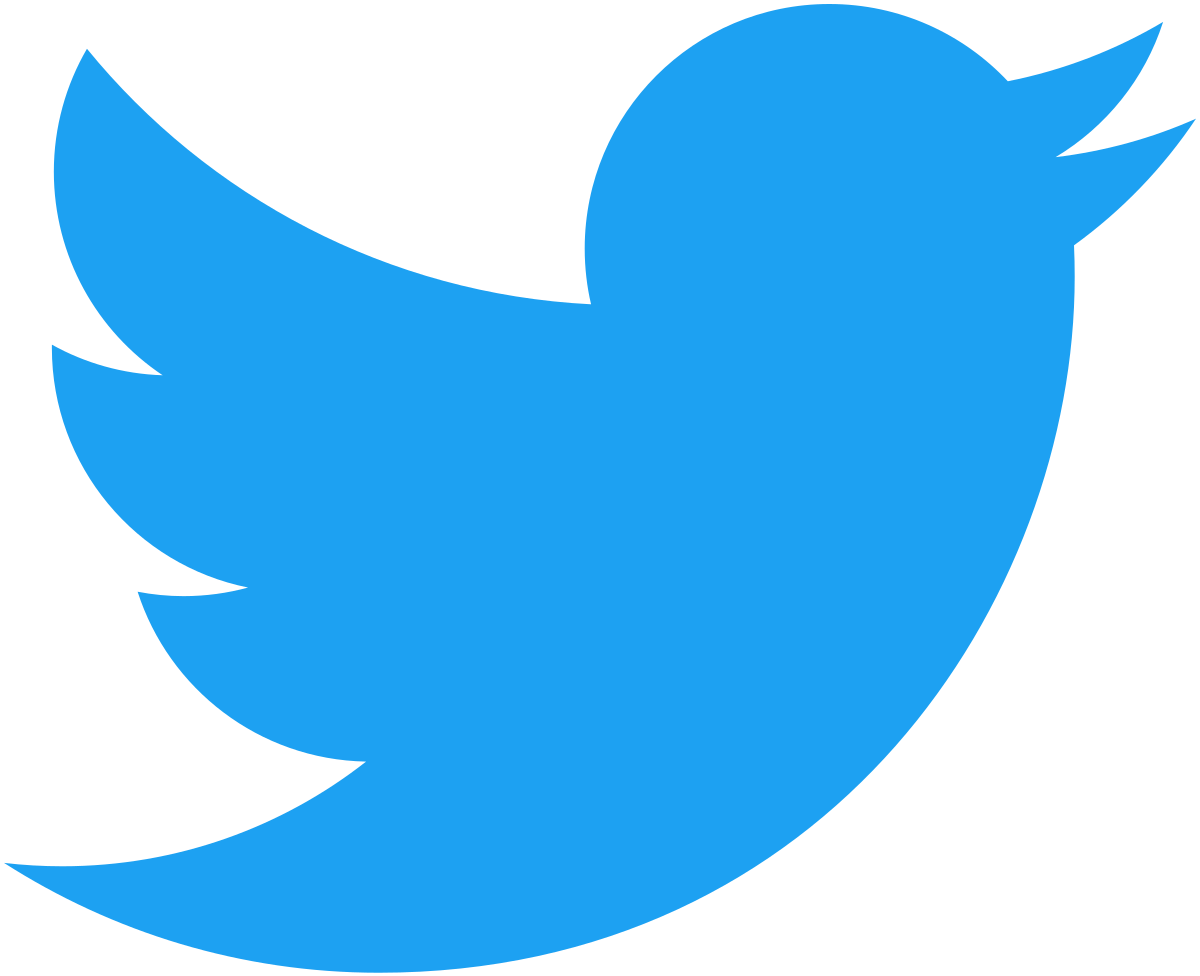
\includegraphics[scale=0.007]{./img/tw_logo.png}   & x       \\ \cline{2-3} 
                                           & 
\includegraphics[scale=0.03]{./img/yt_logo.png}  & \href{https://support.google.com/youtube/answer/9229632}{support.google.com/youtube/answer/9229632}                                  \\ \hline
\multirow{3}{*}{\begin{tabular}[c]{@{}cl@{}}  Fighting \\ misinformation \end{tabular}} & 
\includegraphics[scale=0.05]{./img/fb_logo.png} & \begin{tabular}[c]{@{}cl@{}} \href{https://www.facebook.com/formedia/blog/working-to-stop-misinformation-and-false-news}{facebook.com/formedia/blog/working-to-stop-misinformation-and-false-news}     \\ \href{https://about.fb.com/news/2018/05/hard-questions-false-news/}{about.fb.com/news/2018/05/hard-questions-false-news/}   \end{tabular}                            \\ \cline{2-3} 
                                           & \includegraphics[scale=0.007]{./img/tw_logo.png}   &        \\ \cline{2-3} 
                                           & \includegraphics[scale=0.03]{./img/yt_logo.png}  & \begin{tabular}[c]{@{}cl@{}}  \href{https://www.youtube.com/intl/en\_us/howyoutubeworks/our-commitments/fighting-misinformation/\#policies}{youtube.com/intl/en\_us/howyoutubeworks/our-commitments/fighting-misinformation/\#policies}  \\ \href{https://blog.youtube/inside-youtube/the-four-rs-of-responsibility-raise-and-reduce/}{blog.youtube/inside-youtube/the-four-rs-of-responsibility-raise-and-reduce/}    \end{tabular}                            \\ \hline 
 \end{tabular}
\caption{Summary of ressources, last accessed on July 5, 2021. }
\label{summary}
\end{table*}

\end{landscape}
%https://www.facebook.com/journalismproject/programs/third-party-fact-checking/how-it-works
\end{document}
